\documentclass{report}
\usepackage[utf8]{inputenc}
\usepackage{xcolor}
\usepackage{sectsty} %%Pour changer la couleur de la police 
\usepackage{listings}
\usepackage{amsmath}%%Pour les formules mathématique
\usepackage[final]{pdfpages}%%Pour l'inclusion de PDF
\usepackage{rotating}%%Pour rotation image

\usepackage{float}%%Pour les figures

\title{Rapport}
\author{}
\date{}



\renewcommand{\contentsname}{Table des matières}
\renewcommand{\chaptername}{Chapitre}
\renewcommand{\listfigurename}{Liste des figures}
\renewcommand{\appendixname}{Annexe}
\renewcommand{\bibname}{Bibliographie}


\definecolor{bleurapport}{HTML}{00AAD4}

\chapterfont{\color{bleurapport}}
\sectionfont{\color{bleurapport}}
\subsectionfont{\color{bleurapport}}

\begin{document}


\includepdf{./PageGardeRapportTERM1.pdf}


\newpage
\null %%Pour faire une page vide
\newpage


\section*{Remerciements}
\hspace{0.5cm}Nous tenons tout d'abord à remercier Jimmy Lopez et Sébastien Beugnon pour nous avoir conseillés tout au long de notre projet.
	
	
	Nous remercions aussi nos tuteurs Guillaume Tisserant et Pierre Pompidor pour nous avoir accompagnés tout au long de la réalisation du projet, en particulier pour les choix des méthodes de profilage.

\newpage

%%pour qu'il y ait pas les encadrés rouges mais quand même les liens
            


\tableofcontents %%Table des matières

\newpage

\listoffigures %%Liste des figures

\newpage
\chapter*{Glossaire}

	\textit{Les termes définis dans ce glossaire sont identifiables dans le corps du texte au moyen d'un astérisque (*).}
	\bigbreak
	\begin{itemize}
	
		\item[\textbf{Agressivité : }]	Un joueur agressif va jouer de façon à prendre l'initiative et continuer à miser dans le but d'intimider son adversaire et ainsi prendre l'avantage.	\medskip
		
		\item[\textbf{Blinde : }]Terme correspondant aux mises obligatoires pour les deux joueurs situés à gauche du dealer.\medskip
	
		\item[\textbf{Bluff : }]Le bluff est une technique de jeu qui consiste à jouer comme si l'on possédait un jeu différent de celui détenu en réalité.\medskip	
		
		\item[\textbf{Bouton : }]Le bouton représente le dealer qui distribue les cartes.\medskip
		
		\item[\textbf{Cave : }]La cave correspond à la somme possédée par chaque joueur au début de la partie.\medskip		

		\item[\textbf{Checker : }]Correspond au moment où un joueur reste dans le jeu mais ne place pas d'enchères. Un joueur ne peut checker que si aucun joueur n'a misé avant lui.\medskip
		
		\item[\textbf{Coup : }]Correspond à la distribution courante d'un jeu.\medskip		
		
		\item[\textbf{Dealer : }]Joueur se trouvant sur le siège d'où les cartes vont être distribuées.\medskip		
		
		\item[\textbf{Flop : }]Correspond aux trois premières cartes communes posées sur la table.\medskip
		
		\item[\textbf{IA  : }]Intelligence artificielle.
		
		\item[\textbf{Mise : }]Montant placé sur la table par un joueur à un instant donné.\medskip		
		
		\item[\textbf{Parler :}]Effectuer une action.\medskip
		
		\item[\textbf{Pré-flop : }]Instant du jeu où le joueur possède deux cartes en main avant que les cartes communes n'aient été révélées.\medskip	
		
		\item[\textbf{Profilage : }]	Méthode consistant à établir le comportement d'un joueur, sa façon de jouer.
		
		\item[\textbf{Profilage dynamique : }]Méthode consistant à profiler un joueur tout au long d'une partie, en mettant à jour le profil établi en fonction des actions effectuées.\medskip
		
		\item[\textbf{Profilage statique : }]Méthode consistant à profiler un joueur lors de chaque partie. Le profil établi n'est pas modifié à chaque fois que le joueur profilé effectue une action.\medskip

		\item[\textbf{Rationalité : }]La rationalité  appliquée au poker stipule que toutes les actions d'un joueur ont une logique basée sur les probabilités de gain par rapport à la force d'une main.\medskip

		\item[\textbf{Relancer : }]Une relance correspond au moment où un joueur va miser plus que ce que ses adversaires viennent de miser.\medskip
		
		\item[\textbf{River : }]Cinquième carte commune.\medskip
		
		\item[\textbf{Se coucher : }]Correspond au moment où le joueur abandonne le coup. Ses mises sont alors perdues.\medskip

		\item[\textbf{Turn : }]Quatrième carte commune.\medskip
		
		
		

		
\end{itemize}



\chapter{Introduction}

\section{Généralités}
\hspace{0.5cm}Alors qu'actuellement, de plus en plus de méthodes de profilage sont établies dans le monde des jeux afin de trouver le profil d'un joueur adverse, le poker est un jeu qui pose problème dans ce domaine. En effet, ce jeu est basé sur la chance et sur le bluff. De ce fait, un joueur ne peut jamais être sûr à 100\% de pouvoir gagner et donc, son adversaire ne peut pas deviner le jeu qu'il a de manière certaine. C'est pourquoi, il est dur de profiler un joueur de manière certaine. Il y a donc des recherches dans le développement de méthodes permettant de profiler un joueur de manière efficace. \par

\section{Sujet}
\hspace{0.5cm}Le but de notre projet est de mettre en place une façon de profiler de façon efficace un joueur. Nous devrons tout d'abord établir une méthode de profilage statique. C'est à dire, une technique pour profiler un joueur en fonction des actions qu'il a effectuées pendant toute une partie, de manière globale. Après avoir implémenté cette première méthode de profilage, nous devrons mettre en place une intelligence artificielle pouvant jouer en fonction des résultats obtenus. Ainsi, nous pourrons voir si notre intelligence artificielle est capable de gagner plus de parties une fois le profil du joueur adverse établi. \\
S'il nous reste du temps, nous devrons mettre en place une méthode de profilage dynamique, avec par conséquent, un profil qui s’établit tout au long de la partie et qui est modifié à chaque nouvelle action du joueur adverse. Nous devrons alors, de même que précédemment, mettre en place une intelligence artificielle capable de jouer en exploitant les données de profilage. Ainsi, nous pourrons observer la différence du nombre de parties gagnées en fonction des deux types de profilage, à savoir, statique ou dynamique, mais aussi en fonction des profils établit. En effet, un joueur considéré comme agressif et rationnel est-il plus facile à profil et à battre qu'un joueur considéré comme non agressif et irrationnel ?\par

\section{Rapide description des règles du Texas Hold'Em Poker}
\subsection{Mise en place du jeu}
\hspace{0.5cm}Le Texas Hold'Em Poker est un jeu de cartes dans lequel le but d'un joueur est de gagner le plus d'argent. \par
Afin de commencer une partie, on désigne tout d'abord le bouton* qui sert à désigner le donneur ou dealer*. Le joueur choisi sera donneur pour une main, puis cela sera au tour du joueur à sa gauche une fois cette main terminée et ainsi de suite.  \par

Une fois le donneur sélectionné, il faut poser les blindes*. Le joueur directement à gauche du dealer* pose la petite blinde* alors que celui situé à sa gauche pose la grosse blinde* qui correspond souvent à exactement le double de la petite.\par

Le dealer* doit alors distribuer les cartes aux joueurs, à savoir, deux cartes par joueur. \par

Le jeu se déroule alors en quatre tours d'enchères, à savoir, le préflop*, le flop*, le turn*, et le river*.\par

\subsection{Préflop}
\hspace{0.5cm}Lorsque les cartes ont été distribuées, l'étape préflop* commence. Le tour de mises préflop* démarre donc par le joueur à la gauche de celui ayant mis la grosse blinde*. Celui-ci peut se coucher*, suivre* la grosse blinde* afin de pouvoir rentrer dans le coup ou encore relancer* d'un montant au moins égal à deux fois la grosse blinde*. Le tour d'enchères se termine lorsque chacun des joueurs a eu l'opportunité d'agir et que tous les joueurs qui n'ont pas abandonné ont misé le même montant d'argent dans le pot. Une fois le tour de mises préflop* terminé, on passe à l'étape suivante : le flop.\par

\subsection{Flop}
\hspace{0.5cm}Lors du flop*, le dealer* pose trois cartes faces apparentes au milieu de la table. Le premier tour de mises post-flop commence alors. Les règles sont les mêmes que lors du préflop* mis à part le fait que le premier joueur à parler* peut soit checker* soit miser*.\par

Une fois le tour de mises fini, on passe à l'étape du turn*.\par
\subsection{Turn}
Lors du turn*, le dealer* pose une carte découverte, à la suite des cartes du flop*. \par

Le troisième tour de mises commence alors. Celui-ci est identique au flop*.\par

Une fois celui-ci fini, on passe à la dernière étape, à savoir la river*.\par
\subsection{River}
\hspace{0.5cm}La dernière carte est alors posée par le dealer* au milieu, à la suite des autres cartes découvertes pendant les autres étapes. \par
De même que pour l'étape précédente, un tour de mises est effectué, avec les mêmes règles.\par
Une fois ce tour de mises terminé, les joueurs restants abattent leurs cartes et la meilleure main l'emporte.\par

\subsection{Les combinaisons}
\hspace{0.5cm}Lorsque l'on compare les mains au poker, la main gagnante est celle ayant la combinaison la plus forte. Au poker, il y a 9 combinaisons, de la quinte flush royale, correspondant à la combinaison la plus forte à la carte haute, correspondant à la combinaison la plus faible. Ainsi, une quinte flush royale gagne face à une quinte flush qui elle-même gagne contre un carré et cætera jusqu'à la combinaison la plus faible. \\

Les deux premières combinaisons sont en réalité deux sous-espèces d'une seule et même combinaison, la quinte flush, qui correspond à une suite de cartes de la même couleur.\\

La plus forte des deux, la quinte flush royale est une suite d'une seule couleur, allant de l'as au dix. Par exemple, la main suivante correspond à une quinte flush royale. \par

		\begin{figure}[h]
			\begin{center}
				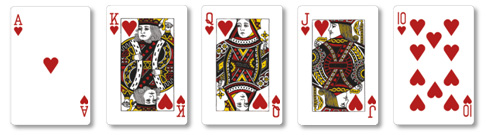
\includegraphics[scale=0.3]{./imagesRapport/quinteFlushRoyale.jpg}
			\end{center}
			\caption[Quinte Flush Royale]{Quinte Flush Royale}
		\end{figure}
		\medskip



La seconde combinaison est composée de toutes les autres suites d'une même couleur, formant une quinte flush, comme on peut le voir dans la figure suivante.\par

		\begin{figure}[h]
			\begin{center}
				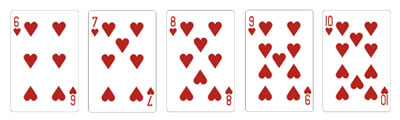
\includegraphics[scale=0.4]{./imagesRapport/quinteFlush.jpg}
			\end{center}
			\caption[Quinte Flush]{Quinte Flush}
		\end{figure}
		\medskip
\newpage
Par la suite, un joueur peut avoir un carré, à savoir, quatre cartes identiques. Si jamais deux joueurs ont un même carré, par exemple si le carré se trouve sur la table, le joueur gagnant sera celui ayant pour cinquième carte la carte la plus haute.\par 

		\begin{figure}[h]
			\begin{center}
				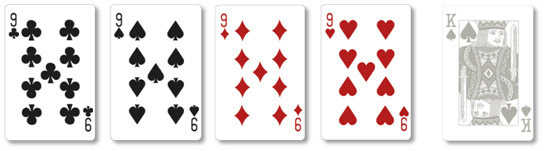
\includegraphics[scale=0.3]{./imagesRapport/carre.jpg}
			\end{center}
			\caption[Carré]{Carré}
		\end{figure}
		\medskip



Après le carré, vient le full qui correspond à trois cartes identiques et deux autres cartes identiques, comme on peut le voir dans la figure 1.4 suivante. \par


		\begin{figure}[h]
			\begin{center}
				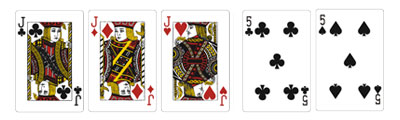
\includegraphics[scale=0.4]{./imagesRapport/full.jpg}
			\end{center}
			\caption[Full]{Full}
		\end{figure}
		\medskip

La combinaison correspondant à une couleur, ou flush, vient ensuite. Un joueur ayant une couleur doit donc avoir une main composée de cinq cartes de la même couleur.\par

		\begin{figure}[h]
			\begin{center}
				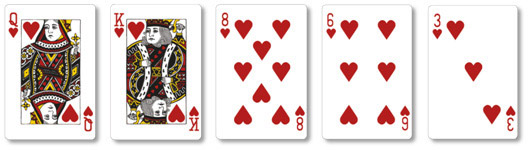
\includegraphics[scale=0.3]{./imagesRapport/couleur.jpg}
			\end{center}
			\caption[Couleur]{Couleur}
		\end{figure}
		\medskip

\newpage
Il y a ensuite une simple suite, donc une main composée de cartes qui se suivent, comme on peut le voir dans l'exemple suivant.\par

		\begin{figure}[h]
			\begin{center}
				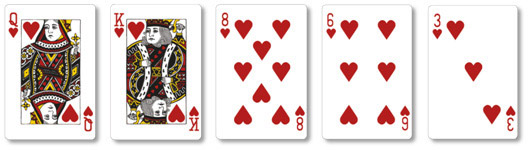
\includegraphics[scale=0.3]{./imagesRapport/suite.jpg}
			\end{center}
			\caption[Suite]{Suite}
		\end{figure}
		\medskip


Lorsqu'un joueur a un brelan, on compte uniquement ses trois cartes. Si jamais il y a égalité entre deux joueurs, on va regarder la carte haute suivante. Si celle-ci a de nouveau le même poids pour les deux joueurs, on regarde la deuxième carte la plus haute. La figure suivante correspond à un exemple de main ayant pour combinaison un brelan.\par
		\begin{figure}[h]
			\begin{center}
				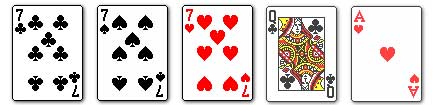
\includegraphics[scale=0.4]{./imagesRapport/brelan.jpg}
			\end{center}
			\caption[Brelan]{Brelan}
		\end{figure}
		\medskip
De même que précédemment, lorsqu'un joueur a une double paire, on compare les paires puis la carte haute. 
		\begin{figure}[h]
			\begin{center}
				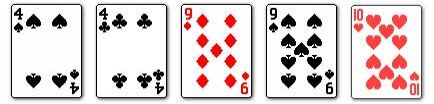
\includegraphics[scale=0.3]{./imagesRapport/doublePaire.jpg}
			\end{center}
			\caption[Double Paire]{Double Paire}
		\end{figure}
		\medskip

De même que pour la combinaison précédente, lorsqu'un joueur a une paire, si jamais il y a égalité entre deux joueurs pour la paire, on va comparer les cartes suivantes, en comparant chaque carte suivante. \par
\newpage
		\begin{figure}[h]
			\begin{center}
				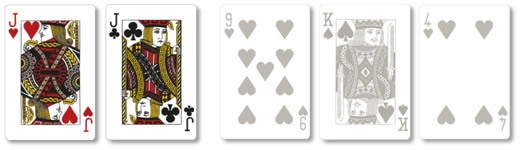
\includegraphics[scale=0.3]{./imagesRapport/paire.jpg}
			\end{center}
			\caption[Paire]{Paire}
		\end{figure}
		\medskip


Enfin, lorsqu'un joueur n'a pas d'autre combinaison, on va regarder sa carte la plus haute. De ce fait, si deux joueurs ont la même combinaison, une carte haute, et qu'ils ont la même carte haute, on va comparer la carte haute suivante et de même jusqu'à ce qu'on ait deux cartes différentes ou alors que l'on ait comparé les cinq cartes de la main. \par
		\begin{figure}[h]
			\begin{center}
				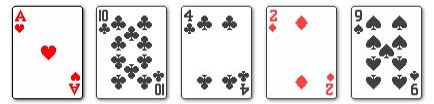
\includegraphics[scale=0.4]{./imagesRapport/carteHaute.jpg}
			\end{center}
			\caption[Carte Haute]{Carte Haute}
		\end{figure}
		\medskip

\section{Cahier des charges}
\subsection{Problématique}
\hspace{0.5cm}Durant les 10 semaines de développement du projet, nous devrons donc implémenter de façon intelligence une simple application permettant de jouer au poker puis, une intelligence artificielle capable de profiler différents types de joueur, tout d'abord de façon dynamique et éventuellement de façon statique. 
\subsection{Fonctionnalités obligatoires}

\hspace{0.5cm}Le projet qui nous a été attribué a pour but de développer une intelligence artificielle de poker permettant d'établir les différents profils des joueurs.\par
L'intelligence artificielle devra donc profiler ses adversaires en se basant sur différents critères comme la rationalité ou l'agressivité. Elle catégorisera alors les différents types de joueurs et leur attribuera des comportements.\\

Il nous est demandé d'établir dans un premier temps un profilage statique basé sur un automate à états finis, qui a pour but d'attribuer un unique comportement à chacun des joueurs pour toute la partie. Ce comportement sera attribué puis modifié après chaque nouvelle partie jouée contre un même joueur.\\

Par la suite, nous devrons mettre en place une nouvelle méthode de profilage afin de profiler de façon dynamique les joueurs. Dans cette seconde version, le profil d'un joueur sera mis à jour tout au long du déroulement d'une partie et l'intelligence artificielle devra pouvoir adapter son comportement aux réactions du joueur adverse.\\

Tout au long du développement, des scénarios de tests seront mis en place afin de vérifier le bon fonctionnement de la catégorisation des joueurs.\par

\subsection{Fonctionnalités optionnelles}

\hspace{0.5cm}Une fois les fonctionnalités obligatoires mises en place, il sera possible d'ajouter la possibilité d'avoir plus de deux joueurs dans une même partie, avec plusieurs intelligences artificielles ou plusieurs joueurs humains mais comprenant toujours au moins une intelligence artificielle.\\

On pourra également intégrer un système de dialogue entre les différents joueurs basé sur des phrases prédéfinies. Ainsi, chaque joueur, humain ou non, pourra envoyer des messages aux autres participants, et notre intelligence artificielle pourra utiliser ces messages pour mieux profiler ses opposants.\par 

\subsection{Spécifications techniques}

\hspace{0.5cm}Afin de faciliter les conditions de travail en groupe, il faudra utiliser un gestionnaire de version.\\

L'application devra être réalisée en utilisant le langage C++ et l'interface sera développée en utilisant Qt.\\

Le développement devra s'appuyer sur les méthodes agiles. Celles-ci sont basées sur une approche itérative dans un esprit collaboratif en prenant compte des besoins des utilisateurs et de leurs évolutions.\par

\subsection{Organisation prévisionnelle}

\hspace{0.5cm}Comme nous pouvons le voir dans l'annexe A représentant le diagramme de Gantt prévisionnel que nous avons mis en place, nous avons prévu dans un premier temps une étude préalable du sujet consistant à nous familiariser avec le vocabulaire du poker. De ce fait, Nous avons rapidement mis en place un glossaire contenant des définitions des différents termes. Pendant cette période, nous avons également défini les besoins des utilisateurs avec entre-autres un diagramme de cas d'utilisations. Nous avons aussi défini comment nous allions nous organiser durant le déroulement du projet, en définissant la fréquence des rendez-vous ainsi que les modalités de partage des données.\\

Par la suite, nous avons prévu de continuer par une étude détaillée durant laquelle nous allons élaborer un diagramme de classe, rédiger le cahier des charges ainsi que commencer à lire des articles sur le sujet.\\

Ensuite, nous passerons à une première étude technique durant laquelle nous commencerons par établir les normes de programmation. Puis, nous développerons une intelligence artificielle simple permettant à un joueur de jouer. Nous réfléchirons par la suite aux différents algorithmes et méthodes permettant d'établir un bon profilage statique du joueur adverse. Et nous établirons des jeux de tests. Dans le même temps, nous commencerons la phase de réalisation, en implémentant en parallèle l'interface graphique et l'intelligence artificielle simple puis, nous ajouterons la méthode de profilage statique et effectuerons les tests définis auparavant.\par
Nous effectuerons ensuite une seconde étude technique pendant laquelle nous définirons les méthodes et algorithmes qui seront utilisés afin d'implémenter la méthode de profilage dynamique. Dans ce même temps, nous implémenterons la méthode de profilage dynamique, en effectuant les tests définis pendant la phase d'étude technique.\\

Enfin, la dernière partie sera réservée à la mise en place de la démonstration qui sera effectuée lors de la soutenance, ainsi qu'à la finalisation du rapport qui sera rédigé tout au long de la période du projet et à la préparation de la soutenance.\par

\chapter{Organisation du projet}



\section{Organisation du travail}

\subsection{Réunions}
\hspace{0.5cm}Comme prévu au départ, nos tuteurs et nous-même avons choisi de nous réunir chaque semaine afin de discuter de nos avancées, des éventuels problèmes rencontrés et des méthodes choisies pour le profilage. De ce fait, nous garantissions que ce que nous faisions était toujours en accord avec les attentes.\\

De notre côté, nous avions choisi de nous réunir chaque mercredi et chaque vendredi matin afin de pouvoir réfléchir ensemble sur les différentes méthodes de calculs. Par exemple, comment déterminer le taux d'agressivité d'un joueur ? Nous nous répartissions ensuite le contenu à implémenter.\\

Étant donné le fait que notre groupe n'était composé que de trois membres, nous avons choisi de ne pas élire de chef de projet mais plutôt de travailler tous sur un pied d'égalité. De ce fait, il n'y a pas eu de spécialisation, chaque membre du groupe a participé à toutes les parties du projet. En effet, notre projet étant basé en particulier sur la réflexion et sur la mise en place de différents algorithmes, il était plus intéressant de travailler à plusieurs.\par

\subsection{Mise en commun du travail}
\hspace{0.5cm}Nous avons choisi d'utiliser un git workflow pour la gestion de notre projet. Cette méthode consiste à mettre en place une branche master qui contient le code de production et sur laquelle rien n'est développé. Elle est donc réservée aux versions fonctionnelles et abouties.
Nous avons ensuite une branche develop sur laquelle sont ajoutées l'ensemble des modifications effectuées au cours du développement et le code qui sera ajouté pour la nouvelle release. Sur cette branche, on peut corriger ou encore améliorer des fonctions. \\

C'est donc une fois l'application dans une version finalisée que sont par la suite ajoutées à la branche master l'ensemble des commits effectués sur le develop.\\

Pour chaque nouvelle fonctionnalité ou correction, nous ajoutions une nouvelle branche en local dans nos répertoires sur laquelle les modifications étaient effectuées. Elles étaient ensuite intégrées à la branche develop en local puis envoyées sur le répertoire public correspondant. Enfin, elles étaient intégrées au répertoire de référence.\par

\subsection{Planification}
\hspace{0.5cm}Le diagramme de Gantt de l'annexe B correspond à la planification réelle de notre projet. Comme on peut vite le constater, nous avons eu du retard et n'avons pas pu finir toutes les tâches prévues au départ. De même, on peut constater que quelques tâches absentes au départ ont été ajoutées.\\

On peut tout d'abord voir que la mise en place de l'interface graphique a pris plus de temps que prévu. En effet, nous n'avions pas prévu que la bibliothèque que nous souhaitions utiliser s’avérerait difficile à mettre en place et que par conséquent il nous faudrait partir de zéro pour l'interface graphique. Étant donné le retard pris pour la mise en place de l'interface graphique, nous avons aussi pris quelques jours de retard sur l'implémentation du jeu de poker et de l'intelligence artificielle basique. \\

Cependant, on peut constater que nous avions commencé l'analyse de l'existant pour le profilage statique bien en avance. Cependant, nous avions ajouté à la liste des articles à lires quelques articles supplémentaires dont une thèse qui nous aura donc pris plus de temps à lire que précédemment. De ce fait, nous avons pris du retard sur la phase d'étude détaillée et sur la phase de développement des algorithmes. De plus, lorsque nous avons voulu passer à la phase d'implémentation des algorithmes. Nous devions récupérer une calculette de probabilités permettant de calculer les chances de gain d'un joueur. Cependant, cette calculette n'ayant pas été retrouvée, nous avons dû ajouter de nouvelles tâches : l'étude détaillée, l'implémentation de la calculette de probabilité et l'implémentation d'un évaluateur de mains. Par conséquent, nous avons mis en pause l'implémentation des algorithmes afin que tous les membres du groupe puissent discuter ensemble de l'étude détaillée de la calculette de probabilités. De ce fait, nous avons pris encore plus de départ dans le déroulement de notre projet. \\

Comme on peut le constater, à mi-parcours du projet, du 31 mars au 10 avril, nous nous sommes rendus compte que la partie concernant le jeu et l'intelligence artificielle était difficilement réutilisable et que l'on découvrait régulièrement des bogues qui n'avaient pas été détectés au moment des tests. Cette partie étant difficilement débogable et nous faisant perdre beaucoup de temps, nous avons choisi de reprendre complètement cette partie. Nous avons perdu beaucoup de temps à ce moment-là et nous nous sommes rendus compte à quel point la découverte tardive d'un bogue fait perdre énormément de temps sur le développement de l'application. Par conséquent, alors que la période d'implémentation des algorithmes liés au profilage statique aurait dû être finie, nous avons repris le code du jeu et avons donc retardé cette implémentation, ce qui a fait prendre du retard aux tâches suivantes.\\

Enfin, nous pensions au départ que nous ne devrions que profiler les joueurs adverses alors que nous devions aussi faire jouer l'intelligence artificielle en fonction du profil établi afin de faire en sorte que l'intelligence artificielle gagne le plus d'argent possible. De ce fait, nous avons ajouté les tâches en rapport à la mise en place du jeu de l'intelligence artificielle en fonction des profils établis. \\

Nous pouvons donc en conclure que nous avons pris beaucoup de retard, sûrement à cause du fait que nous n'avions pas bien compris l'ampleur des tâches qui seraient à effectuer et à cause d'une mauvaise conception au départ de la partie correspondant au jeu et à l'intelligence artificielle basique. Finalement, étant donné que l'on s'est rendu compte du retard pris sur le projet, plutôt que terminer précipitamment la partie sur le profilage statique pour commencer le profilage dynamique prévu, nous avons préféré ne pas nous précipiter et terminer correctement le profilage statique et obtenir de bons résultats, quitte à ne pas faire la partie dynamique. \par

\section{Méthodes et outils de travail}
\subsection{Gestionnaire de versions}
\hspace{0.5cm}Notre choix s'est porté sur le gestionnaire de version Git, car contrairement à d'autres tels que Subversion, Git est décentralisé. Il ne repose pas sur un seul et même dépôt en ligne sur lequel chaque nouvelle version d'un fichier envoyée remplace la précédente et affecte donc l'ensemble du groupe. Git met en place, en plus du dépôt de référence commun à tous, un dépôt en ligne et un dépôt local pour chacun des utilisateurs, comme on peut le voir dans le schéma suivant.\par
\begin{figure}[H]
	\begin{center}
			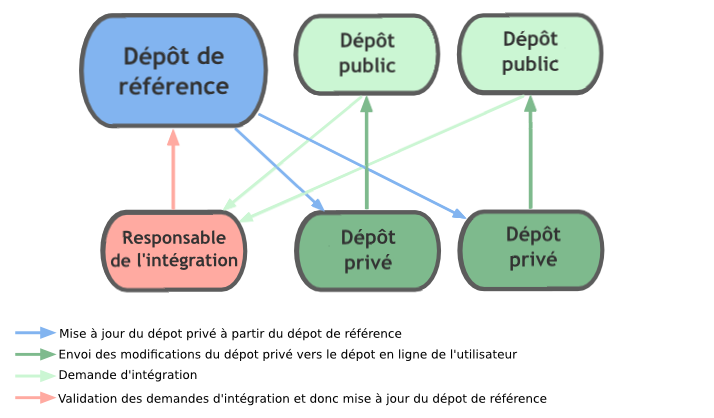
\includegraphics[scale=0.6]{./imagesRapport/schemaGit.png}
	\end{center}
	\caption[Schéma de fonctionnement de Git]{Schéma de fonctionnement de Git}
\end{figure}
\medskip
					 L'utilisation de dépôts publics, en vert clair sur le schéma, permet d'éviter les conflits, notamment lorsque deux personnes travaillent sur un même fichier, puis souhaitent l'envoyer sur le dépôt commun simultanément. Ici, les fichiers sont envoyés sur les dépôts en ligne personnels, puis intégrés sur le dépôt de référence, représenté en bleu, par la personne en charge lorsque les utilisateurs effectuent une demande d'intégration auprès du responsable (integration manager).\\
				
	Les conflits n'ont lieu dans ce cas, que lorsqu'une même ligne est modifiée plusieurs fois, auquel cas, c'est le responsable d'intégration qui le verra et donc n'acceptera pas les modifications proposées.

\subsection{Normes de programmation}
\hspace{0.5cm}Concernant la réalisation du projet, l'application sera développée en français. Par conséquent, les différents identifiants des attributs, noms de classes et fonctions/méthodes que nous implémenterons auront des noms français, les méthodes toString ainsi que pour les accesseurs et mutateurs que nous nommerons getNomAttribut et setNomAttribut, selon les conventions de codage établies.\\

Les noms des classes commenceront toujours par une majuscule suivie de minuscules. Si le nom de la classe est composé de plusieurs mots, alors on ajoutera une majuscule à chaque début de mot.\\

Les noms des méthodes, des variables et des attributs devront impérativement commencer par une minuscule avec une majuscule à chaque nouveau mot.\\

Pour l'indentation, il faudra mettre un maximum d'accolades, facilitant la reprise et l'ajout de code, même lorsque celles-ci ne sont pas obligatoires.\\

Des commentaires seront ajoutés pour chaque fonction et méthode, au dessus de la déclaration correspondante, dans les fichiers d'en-tête. Les commentaires des accesseurs et mutateurs ne sont pas obligatoires car explicites.
Dans ces commentaires seront précisés l'action de la fonction/méthode, l'ensemble des paramètres, l'élément retourné s'il existe. Ces commentaires seront de la forme suivante : \par

\begin{lstlisting}
/**
 *  @param
 *  @action
 *  @return
**/
\end{lstlisting}

\newpage

Au début de chaque nouveau fichier créé, il faudra ajouter l'en-tête suivante: 
\begin{lstlisting}
/*===============================================
Nom: fichier.cpp         Auteur: 
Maj:  27/03/2014         Creation: 01/02/2015
Projet: Profilage par essais et erreurs au poker
-------------------------------------------------
Specification: Specifications du fichier
=================================================*/
\end{lstlisting}

De plus, chaque commit effectué sur le projet Git devra avoir une description explicite permettant de savoir, sans avoir à parcourir le code, les modifications qui ont été apportées.\par

\chapter{Analyse du projet}

\section{Analyse de l'existant}


%%TODO: trouver comment on fait référence à un article ds un rapport 
%%      reprendre le texte
%%      ajouter plus de références / expliquer en quoi on s'est servi des                                                                  articles

\hspace{0.5cm}Avant de commencer à réfléchir aux différentes méthodes de profilage, nous avons choisi de lire différents articles sur le sujet pour nous faire une idée des données à prendre en compte et des différentes méthodes que nous pourrions utiliser. \\

Malgré la lecture des articles, nous avons choisi de développer nos propres méthodes de profilage, sans utiliser exactement les calculs décrits dans les différents articles. Cependant, nous avons quand même choisi de nous inspirer des articles, notamment pour le choix des paramètres importants à prendre en compte, par exemple pour le calcul du profil du joueur, à savoir, le taux d'agressivité, de rationalité, de passivité et de bluff. \\

Ainsi, grâce à l'article "Poker as a Testbed for IA Research", expliquant entre-autres les paramètres à prendre en compte pour avoir une base de jeu solide, nous avons isolé de façon plus rapide les paramètres importants pour établir les profils des joueurs. De ce fait, nous en avons déduit que le paramètre à prendre en compte en priorité est la force de la main et qu'il faudra bien entendu la recalculer à chaque nouvelle étape puisque suite à l'apparition de nouvelles cartes, les chances de gain d'un joueur peuvent complètement changer. De même, nous nous sommes basés sur l'article pour la façon dont notre intelligence artificielle allait jouer pour gagner. En effet, dans cet article, il est expliqué à quel point il est important d'avoir un jeu imprévisible, c'est à dire de ne pas effectuer toujours les mêmes actions. \\

Cependant, nous ne nous sommes pas seulement inspirés de l'article présenté précédemment. En effet, cet article ne se concentre que sur la force de la main, le potentiel d'une main ainsi que la stratégie de jeu et ne traite pas de façon précise des paramètres à prendre en compte pour profiler un joueur. \\

Pour choisir les paramètres à prendre en compte pour le profilage d'un joueur, nous nous sommes inspirés de la thèse "Probabilities and Simulations in Poker". En effet, dans cette thèse, Maria de Lourdes Peña Castillo explique que pour profiler de manière efficace un joueur, il faut se baser sur le triplet suivant, le taux de suivis, de mises et de checks. \\

Par la suite, si nous avons lu beaucoup d'articles traitant de la mise en place d'une table de poids pour calculer la possible main d'un adversaire en fonction de ses actions, notamment la thèse "Probabilities and Simulations in Poker" ou encore l'article "Player Profiling in Texas Hold'em Poker". Cependant, au vu de la complexité de la mise en place de ce calcul, nous avons choisi de mettre de côté l'implémentation de cette fonctionnalité et de la reprendre éventuellement si nous avions du temps à la fin. \\



%%Présenter les articles

%%Ebauches d'infos sur ce qui est contenu par les articles
%
%Articles parlant de la table de poids :
%Improved Opponent Modeling in Poker
%Player Profiling In Texas Holdem
%
%Table de frequence de "paris" : 
%Improved Opponent Modeling in poker
%
%Facteurs à prendre en compte pour le profilage :
%Improved Opponent Modeling : montant pot
%
%
%Poker as a testbed for AI research (Loki-1):
%- force main calculée au flop, turn et river
%- stratégie : déterminer quelle action est la meilleure
%			prendre en compte : -force main
%								-profil établi
%- profil adversaire : faible/fort agressif/passif
%
%
%
%Probabilities and simulations in poker (Loki-1 et Loki-2):
%- profilage dynamique : triplets de proba : fold,call,raise
%- table de poids (OM)

\section{Système de jeu}

\subsection{Deux joueurs}
\hspace{0.5cm}Afin de pouvoir effectuer le profilage d'un joueur, nous avons mis en place un jeu de poker à deux joueurs. Dans un premier temps, il s'agissait d'un joueur humain contre une intelligence artificielle ayant pour but de le profiler. Pour pouvoir jouer, une interface graphique a été mise en place pour permettre à la fois le suivi de la partie et le choix des actions.\\

Au départ, l'intelligence artificielle reposait sur un algorithme basique lui permettant de jouer une partie. Puis nous avons rapidement mis en place un calibrage de l'intelligence artificielle, afin de pouvoir lui attribuer un style de jeu (agressif, rationnel...). Lors de l'ajout de ce calibrage, nous avons complexifié le jeu de l'intelligence artificielle en prenant en compte le calibrage donné mais aussi en y ajoutant un choix d'action plus varié.\\

Afin de différencier les joueurs profilés, nous avons mis en place un système de pseudos. Avant le démarrage du jeu, il est alors possible de renseigner un pseudo, nouveau ou déjà existant, qui permet à l'intelligence artificielle de collecter et rassembler les données de profilage d'un même joueur. De ce fait, s'il se déconnecte et souhaite rejouer un autre jour, l'intelligence artificielle disposera toujours du précédent profilage effectué.\par

\subsection{Intelligence artificielle contre intelligence artificielle}
\hspace{0.5cm}Par la suite, afin de permettre l'automatisation du profilage, et le lancement d'une série de parties, il nous a été demandé de revoir le système de jeu afin que l'intelligence artificielle existante puisse jouer contre une deuxième intelligence artificielle ne profilant pas. Dans cette version, l'interface n'est plus prise en compte et les deux intelligences jouent simultanément jusqu'à fin de la partie. Dans ce cas, un calibrage est donné pour cette deuxième intelligence artificielle, et celui-ci reste fixe pour la suite de parties. C'est l'intelligence artificielle qui profile qui va tenter de retrouver les valeurs de ce calibrage.\\

Pour permettre ces séries de tests, nous avons donc ajouté la possibilité de choisir le nombre de parties à lancer, afin de tester de façon efficace le profilage mis en place et déterminer la façon optimale d'établir le profil du joueur adverse.\par

\subsection{Choix d'enregistrement des données}

\hspace{0.5cm}Afin de profiler les joueurs, nous avons choisi d'enregistrer un certain nombre de données dans des fichiers de sortie. Selon le système de pseudos développé, nous avons décidé de mettre en place un fichier par joueur, représenté par le pseudo du joueur ou bien son calibrage dans le cas d'une intelligence artificielle. Dans le but d'une réutilisation des données enregistrées par l'application, nous avons au départ choisi le format de données Json car il a l'avantage d'être facilement exploitable. De plus, nous avons pu utiliser la librairie QJson pour traiter les données des fichiers.\\

Nous avons ensuite déterminé les données à prendre en compte au cours d'une partie, qui permettront le profilage du joueur adverse, et qui seront enregistrées dans les fichiers json.\par
On enregistre chaque valeur est représentée sous forme de taux, en pourcentage.\\

Au cours d'une partie, l'intelligence artificielle va enregistrer les chances de gain du joueur, calculées en fonction des cartes du joueur adverse en fin de partie.\\

Elle va également calculer les différentes actions effectuées. Ici, nous avons choisi de classer les différentes actions en trois catégories, les suivis, les checks, et les mises qui comprennent aussi les relances. Chacune de ces valeurs représente donc le pourcentage de réalisation de cette action par le joueur en fonction du nombre de tours de jeu (par exemple si le joueur a suivi une fois sur deux, on aura 50\% de suivis). Si le joueur ne se couche pas, le total de ces trois valeurs est donc 100\%. Enfin un booléen indique si le joueur s'est couché ou non au cours de la partie.\\

Concernant les mises, afin d'être plus précis sur l'agressivité du joueur, nous mémorisons également la mise la plus haute effectuée en une fois par le joueur, ainsi que le total du montant misé sur l'ensemble des tours.\\

Finalement, le fichier contient tous les types de comportements possibles que l'on peut attribuer au joueur profilé. Nous avons choisi de catégoriser le joueur selon quatre critères : l'agressivité, c'est à dire sa capacité à miser, la rationalité, le bluff et la passivité. Ces quatre valeurs sont exprimées en pourcentage. Pour chacune d'elle nous avons déterminé une formule qui, à partir des données enregistrées dans le fichier et présentées plus haut, va calculer les taux associés.\\

Enfin, dans le but d'effectuer un profilage plus précis des joueurs, nous avons distingué chaque étape de jeu, et donc enregistré l'ensemble de ces valeurs pour les quatre étapes d'une partie : préflop, flop, turn et river. Un profil global de la partie est ensuite écrit avec les quatre valeurs de comportement. Puis un booléen contient le résultat de la partie.\\

Finalement, nous nous sommes rendu compte qu'enregistrer les différentes valeurs utile au profilage en fonction de chaque étape n'était pas optimal. En effet, un profil calculé globalement donnait des résultats plus cohérents qu'un profil calculé à chaque étape d'une partie. Nous avons donc choisi d'enregistrer uniquement les données de manière globale.\\


Par la suite, nous avions besoin de créer des graphes avec les données enregistrées dans les fichiers de sortie. Nous nous sommes alors rendus compte que l'utilisation de fichiers de type csv était plus adaptée. De ce fait, nous avons décidé de changer le type de nos fichiers de sortie en csv.\\

Nous avons ensuite ajouté le gagnant de la partie, ainsi que les gains ou pertes d'argent de l'intelligence artificielle au cours de la partie. De cette manière, il nous serait facilement possible d'observer les gains cumulés de l'intelligence artificielle au bout de plusieurs parties et en faire un graphique.\par


\section{Profilage}
\hspace{0.5cm}Pour établir le profil d'un joueur, nous nous basons sur quatre taux qui seront établis en fonction du comportement du joueur adverse.\\

Nous prenons d'abord en compte la rationalité du joueur, c'est à dire si le montant de ses mise ou bien ses actions sont en accord avec son jeu. Pour calculer ce taux, nous nous basons donc sur les chances de gain du joueur ainsi que sur le montant total de ses mises au cours de la partie. Comme on ne connaît pas durant la partie les cartes du joueur adverse, le taux de rationalité est calculé uniquement à la fin de la partie, après avoir déterminé le gagnant, une fois les cartes du joueur profilé visibles.\\

Le second critère pris en compte est l'agressivité, qui correspond à la capacité d'un joueur à prendre l'initiative et continuer à miser sans forcément prendre en compte son jeu, dans le but d'intimider son adversaire et ainsi prendre l'avantage. Les données qui seront prises en compte sont l'ensemble des mises du joueur. C'est à dire, le total des mises, la mise la plus haute ainsi que le nombre de mises effectuées durant la partie. \\

Il faut aussi prendre en compte la passivité d'un joueur, c'est à dire, si le joueur a tendance à suivre son adversaire plutôt qu'à prendre les devants. Pour cela, nous prenons en compte le nombre de suivis et le nombre de checks effectués tout au long de la partie par le joueur profilé.\\

Enfin, le critère du bluff est à prendre en compte. Un joueur bluffeur est un joueur qui va effectuer des actions qui ne sont pas en accord avec ses chances de gain. On part donc du principe qu'un joueur bluffeur est un joueur irrationnel.\\

Ces quatre valeurs vont nous permettre d'établir le profil d'un joueur au cours d'une partie. Elles seront mises à jour à chaque partie pour un profilage statique et à chaque tour de jeu pour un profilage dynamique. \\

Pour établir le profil global d'un joueur, avoir les données sur une partie n'est pas suffisant. Il faudra donc que l'intelligence artificielle joue plusieurs parties contre le joueur afin d'en déduire le profil global. Nous lancerons donc, pour chaque nouvel adversaire plusieurs parties pour établir leur profil puis, nous pourrons commencer à jouer de manière efficace une fois ce profil connu.\\

Dans le cadre du TER, nous nous sommes concentrés sur le profilage statique afin qu'il soit le plus juste possible. Les parties suivantes traiteront donc uniquement du profilage statique. \par


\section{Phase de jeu}

\hspace{0.5cm}Le but de l'intelligence artificielle qui profile est d'établir un profil pour pouvoir ensuite l'utiliser comme référence afin de tenter de gagner un maximum de parties et de jetons. Après la phase de profilage, il y a donc la phase de jeu. Durant cette phase, l'intelligence artificielle ne profile plus le joueur adverse, pour tenter d'augmenter ses gains. Durant cette phase, si l'intelligence artificielle commence à trop perdre alors, la phase de profilage est relancée. En effet, le trop grand nombre de pertes peut être dû à un mauvais profil établi. \\



\chapter{Mise en place du jeu et de l'interface graphique}
\section{Jeu}
%%Faire diagramme de classe avec le jeu et IA dedans
\section{Interface graphique}
%%Faire un diagramme de classe de l'interface avec contenu fenetre IA et humain
\subsection{Intelligence artificielle face à un joueur humain}
\subsection{Intelligence artificielle face à une autre intelligence artificielle}

\chapter{Calcul du profil d'un joueur}


\hspace{0.5cm}Dans le but d'implémenter le profilage d'un joueur, nous avons établi les formules de calcul de chacun des comportements. \par

\section{Rationalité}

\hspace{0.5cm}Afin de calculer le taux de rationalité d'un joueur pendant une partie, nous avons choisi de nous baser sur une courbe correspondant aux pourcentages théoriques de rationalité en fonction des chances de gagner. 

\begin{figure}[H]
	\begin{center}
		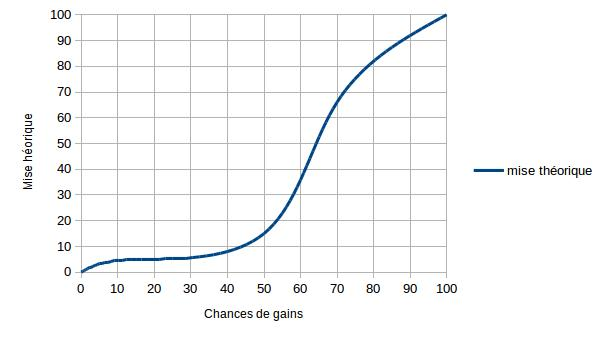
\includegraphics[scale=0.5]{./imagesRapport/courbeRationaliteMiseTheorique.jpg}
	\end{center}
	\caption[Mise théorique en fonction de la rationalité]{Mise théorique en fonction de la rationalité}
\end{figure}

La figure ci-dessus représente la courbe sur laquelle nous nous basons pour calculer le pourcentage de jetons qu'un joueur devrait théoriquement miser par rapport à la cave de départ, en fonction de ses chances de gain. Ainsi, on peut voir qu'au départ, un joueur rationnel ne doit presque rien miser, à savoir pas plus de 15\% de ses jetons, puis, à partir du moment où ses chances de gain sont supérieures à 50\%, il doit commencer à miser beaucoup, de façon proportionnelle à ses chances de gain.\\

A partir de cette courbe, nous avons décidé de calculer la mise que le joueur aurait dû théoriquement mettre en jeu en nous basant sur quatre paliers, comme nous pouvons le voir dans la formule suivante. \par

\small{
 	Gain = chances de gain du joueur,\\
Ra = rationalité\\
$M_{th}$ = Mise théorique.\\

\begin{align*}
	\hspace{-1cm}M_{th} = \left((Gain - g1) * \left(\frac{m2-m1}{g2-g1}\right)\right)+m1
	\begin{cases}
		Ra \in [m1=0 - m2=10] &\text{Si Gain} \in [g1=0 - g2=30]\\
		Ra \in [m1=11 - m2=25] &\text{Si Gain} \in [g1=31 - g2=50]\\
		Ra \in [m1=26 - m2=65] &\text{Si Gain} \in [g1=51 - g2=69]\\
		Ra \in [m1=66 - m2=100] &\text{Si Gain} \in [g1=70 - g2=100]\\
	\end{cases}
\end{align*}
}

Pour chaque palier, on regarde si les chances de gain du joueur sont comprises entre g1 et g2. Une fois le palier trouvé, on calcule la mise théorique, en sachant que celle-ci sera comprise entre les m1 et m2 correspondant au palier. \par
Dans chacun de ses paliers, on calcule donc la mise théorique dans le palier correspondant, de façon proportionnelle aux chances de gain du joueur. Par exemple, 15\% de chances de gain vont donner 5\% de mise théorique.\\
	
Après avoir calculé la mise théorique, nous la comparons avec la mise réelle du joueur. La rationalité s’obtient alors avec la formule suivante. \par

\begin{align*}
Rationalit\acute{e} = 100-abs(M_{th}-M_{r\acute{e}elle})
\end{align*}



\section{Agressivité}

\hspace{0.5cm}Pour calculer le taux d'agressivité d'un joueur, nous nous sommes basés sur le même système de paliers que pour la rationalité. Nous prenons en compte trois paramètres, qui sont le taux de mises ainsi que le total des mises et la mise la plus haute, exprimés en en pourcentage de jetons par rapport à la cave de départ. Ici, nous allons donc établir une formule à partir des trois paramètres listés précédemment.\\

Au départ, nous avions décidé que le critère le plus important serait la mise la plus haute. Cependant, nous nous sommes vite aperçus que ce n'était pas le critère le plus représentatif de l'agressivité. Par conséquent, la formule met maintenant en avant le total des mises effectuées.\\

Chaque palier est donc déterminé par le total des mises du joueur. De ce fait, le palier correspondant est celui pour lequel la mise totale est comprise entre les bornes inférieures et supérieures. Le taux d'agressivité théorique est alors calculé en fonction du palier correspondant et des deux autres paramètres, nombre de mises et mise la plus haute, qui ont pour ratios, respectivement ratio1 et ratio2. \\

\small{
\begin{align*}
	Ag_{th}=
	\begin{cases}
		Ag_{th} \in [0-50] Si mtot \in [0-25] &\text{ratio1}=\frac{1}{2} \text{ ratio2}=\frac{1}{2} \\
		Ag_{th} \in [51-80] Si mtot \in [26-50] &\text{ratio1}=\frac{2}{3} \text{ ratio2}=\frac{1}{3} \\
		Ag_{th} \in [81-100] Si mtot \in [51-100]  &\text{ratio1}=\frac{2}{3} \text{ ratio2}=\frac{1}{3}\\
	\end{cases}
\end{align*}
}


Le calcul de la mise théorique d'agressivité se base sur la mise totale du joueur à laquelle on ajoute les deux autres critères avec les poids correspondant aux ratios présentés précédemment. \par
\begin{align*}
	&0<y<mph2-ag2\\
	&x=ratio1 * nbMises + ratio2 * miseLaPlusHaute\\
	&y=\left(x*\frac{mph2-ag2}{100}\right)
\end{align*}


Pour le dernier palier, nous ne nous basons pas sur la formule précédente mais sur la formule suivante :\\ 

\begin{align*}
	y=\left(x*\frac{100-mph}{100}\right)
\end{align*}

Finalement, l'agressivité est calculée comme suit. 

\begin{align*}
	y=\left(mtot + y\right)
\end{align*}

\section{Bluff}

\hspace{0.5cm}Étant donné le fait que nous partons du principe que le bluff est l'inverse de la rationalité, nous calculons le taux de bluff en utilisant la formule suivante : \par

\begin{align*}
	bluff=100-rationalit\acute{e}
\end{align*}


\section{Passivité}

\hspace{0.5cm}Nous avons décidé que le taux de passivité d'un joueur se calcule en fonction du nombre de ses actions check et suivre.\par
\begin{align*}
	passivit\acute{e}=tauxChecks+tauxSuivis
\end{align*}


\chapter{Intelligence artificielle}
\section{Résolveur}
\subsection{Résolveur basique}


Étant donné le fait que nous devions rapidement avoir une simple intelligence artificielle pour commencer à profiler le joueur adverse, nous avons commencé par implémenter une intelligence artificielle basique, ne se basant que sur ses chances de gain au préflop.\\

Nous regardions donc tout d'abord si les chances de gain étaient supérieures à 75\%. Si c'était le cas, l'intelligence artificielle se mettait alors à jouer de façon très agressive, en misant, relançant ou parfois même en faisant tapis dès que possible.\\

Si la force du jeu de l'intelligence artificielle était supérieure à 50\%, l'intelligence artificielle suivait ou misait selon l'action possible.\\

Enfin, si les chances de gain étaient inférieures à 50\%, l'intelligence artificielle avait le choix entre les actions suivre, checker ou encore se coucher si jamais le montant nécessaire pour rester en jeu était trop important. Notre intelligence artificielle était donc rationnelle mais n'était pas paramétrable, ce qui par la suite devait être corrigé. \par
C'est pourquoi nous avons ensuite modifié son implémentation afin de pouvoir lui associer un comportement.\par


\subsection{Résolveur avec calibrage}

\hspace{0.5cm}Afin de pouvoir tester facilement notre profilage, et pouvoir faire varier les actions des intelligences artificielles, nous devions pouvoir choisir le comportement de chaque intelligence artificielle. Pour cela, nous avons permis le calibrage de l'intelligence artificielle, à partir d'un taux d'agressivité et un taux de rationalité donné. Une intelligence artificielle agressive aura donc tendance à fortement miser.\\

Pour cela, nous devions donc faire en sorte que les actions choisies par le résolveur soient en accord avec les taux d'agressivité et de rationalité donnés. Nous avons donc choisi de mettre en place une liste d'actions possibles pour une action agressive et de même pour une action rationnelle. Après avoir calculé les actions d'agressivité et de rationalité, nous faisions par la suite un choix entre les deux actions, afin d'avoir des actions cohérentes par rapport aux deux taux. Nous détaillerons par la suite la façon dont nous avions implémenté le choix des différentes actions et la méthode de fusion.\\

Pour notre première version du calibrage, nous avons choisi de calculer une action pour chaque paramètre du calibrage, donc une action d'agressivité et une action de rationalité. Puis nous avons mis en place une méthode de sélection à partir des deux actions calculées et des taux de calibrage correspondants.\\

Pour le choix de l'action agressive, le calcul se base sur une mise théorique d'agressivité en fonction des mêmes paliers établis que pour le profilage. Puis, afin de respecter le pourcentage d'agressivité donné à l'intelligence artificielle, nous avons dans un premier temps pensé à alterner entre action agressive et action passive en fonction du calibrage. En effet, le profilage de l'agressivité s'effectue selon trois critères : la fréquence de mises, la mise la plus haute et le montant total des mises. De ce fait, afin que notre intelligence artificielle ne mise pas de façon constante, nous avons pensé à générer un nombre aléatoire entre un et cent et le comparer au taux d'agressivité donné pour choisir l'action. Par exemple, si le calibrage d'agressivité vaut 70\%, alors si le nombre aléatoire est compris entre 0 et 70, on effectue une action de mise cohérente selon la mise théorique (une mise, une relance ou un suivi selon la situation), et si au contraire le nombre est compris entre 70 et 100, on choisit une action passive.\\



Le choix de l'action rationnelle était basé sur le même principe. La mise théorique de rationalité est calculée en fonction des chances de gain de l'intelligence artificielle, puis de la même manière que pour l'agressivité, un nombre aléatoire détermine si on effectue une action rationnelle ou non. Si on a une valeur de rationalité entre zéro et le taux, alors on choisit une action rationnelle, qui correspond à la mise théorique et qui varie selon la situation actuelle du jeu. Sinon, on liste l'ensemble des actions irrationnelles, comme une mise en dessous ou en dessus de la mise théorique, puis pour renforcer l’irrationalité, et donc l'imprévisibilité du joueur, la sélection de l'action parmi toutes celles considérées comme irrationnelles se fait de façon aléatoire.\\

Enfin, une fois les deux actions calculées, une sélection aléatoire est faite entre ces deux actions, avec les chances de sélection proportionnelles aux valeurs de calibrage.\\

Par la suite nous avons revu le calibrage de l'agressivité qui n'était pas assez précis. En effet, comme pour calibrer la rationalité, nous laissions une part de hasard dans le calcul de l'action de l'intelligence artificielle. Ceci avait pour effet de produire des résultats parfois trop éloignés du calibrage de départ.\\

Pour pallier ce problème, nous avons mis en place le calcul d'une action de mise correspondante au taux d'agressivité en fonction de la mise totale effectuée par l'intelligence artificielle au cours de la partie. Nous avons également adapté le calcul côté profilage afin que la mise totale devienne le critère principal, à la place de la mise la plus haute.
A chaque tour, le résolveur calcule donc la mise théorique à effectuer selon les nouveaux paliers.\par


\begin{figure}[H]
\begin{center}
\begin{tabular}{|l|l|}
	\hline
   Agressivité & Mise totale \\
   \hline
   0 – 50 & 0 – 25	exclu \\
   \hline
   50 – 80 & 25 – 60 exclu\\
   \hline
   80 – 100 & 60 – 100 exclu\\
   \hline
   100 & 100\\
   \hline
\end{tabular}	
\end{center}
\caption{Paliers d'agressivité et mise totale en fonction}
\end{figure}

Selon le calibrage, le but est donc que l'intelligence artificielle effectue la mise prévue. Seulement, il n'est pas possible de déterminer la durée de la partie. Il faut donc que celle-ci effectue progressivement sa mise, sans terminer trop tôt où elle devra effectuer des actions check ou suivi pour terminer, ce qui diminuera le taux d'agressivité, et ni trop tard pour qu'elle puisse être considérée suffisamment agressive.\\

Pour ce faire, nous misons de façon croissante, depuis un départ minimum, jusqu'à atteindre la mise théorique totale calculée à partir du calibrage.\par
En prenant un rapport $\times2$, on obtient donc les mises totales suivantes à chaque tour de jeu.\par

\begin{figure}[H]
\begin{center}
Exemple : 	5 – 10 – 20 – 40 – 80 		avec 80 mise totale théorique.
\end{center}
\end{figure}
Dans ce cas, cela revient donc à miser 5; 5; 10; 20 puis 40.

Afin d'obtenir ce résultat, nous différencions deux cas : celui où l'intelligence artificielle peut miser et celui où elle doit suivre/relancer ou se coucher.\par
Si elle peut miser, alors elle joue la mise théorique courante en faisant attention de ne pas dépasser la mise théorique totale. Dans le cas où on est au river (dernier tour), alors elle mise directement ce qui lui manque pour arriver à cette mise théorique totale.\\

Dans le cas où l'adversaire a misé/relancé, alors l'intelligence artificielle va comparer la mise théorique courante avec la mise adverse et la valeur de relance minimum. Dans le cas où le mise théorique est inférieure à la valeur de suivi -10\% alors on se couche, pour ne  pas miser trop haut en suivant. Si celle-ci est comprise entre le taux de suivi $\pm$ 10\%, on suit.
Dans le cas où la relance est inférieure ou égale à la valeur à miser +10\% , on relance de la valeur la plus proche de la mise théorique. Sinon on suit.\\


A la suite de ces changements nous avons également revu la sélection entre les actions d'agressivité et de rationalité, une fois ces deux dernières calculées.\par

Une fois que le calibrage nous a donné l'action agressive et l'action rationnelle, on effectue une fusion entre les deux. Dans les cas où les deux actions sont identiques, l'action est prise. Si ce sont toutes les deux des mises/relances, on prend la moitié du nombre de jetons, proportionnellement aux pourcentages de calibrage.\\

Le tableau suivant présente des exemples de combinaisons possibles, avec par conséquent des actions agressives et rationnelles différentes ainsi que l'action finale déduite.\\


\begin{figure}[H]
\begin{center}
\begin{tabular}{|l|l|l|}
	\hline
	Action agressive		&	Action rationnelle 	&	Action finale\\
	\hline
	Checker		&	Se coucher	&	Checker\\
	\hline
	Checker		&	Suivre		&	Tirage aléatoire\\
	\hline
	Checker		&	Miser		&	Miser (fusion)\\
	\hline
	Suivre		&	Relancer		&	Si montant > relance minimum, Relancer\\
				&				&		Sinon, Suivre\\
	\hline
	Suivre		&	Se coucher	&	Tirage aléatoire\\
	\hline
	Relancer		&	Se coucher	&	Suivre\\
	\hline
	Miser		&	Se coucher	&	Miser (fusion)\\
	\hline
	Tapis		&	Miser		&	Miser (fusion)\\
	\hline
	Tapis		&	Relancer		&	Relancer (fusion)\\
	\hline
	Tapis		&	Se coucher	&	Si peut suivre, Suivre\\
				&				&	Sinon, Miser cave/2\\
	\hline
	Tapis		&	Checker		&	Si peut suivre, Suivre\\
				&				&   Sinon, Miser cave/2\\
	\hline
\end{tabular}
\end{center}
\caption{Choix de l'action à effectuer en fonction des actions d'agressivité et de rationalité}
\end{figure}

Si l'on considère une intelligence artificielle ayant un taux d'agressivité égal à  70\% et un taux de rationalité égal à 20\%, et des actions de mises choisies dans chacun des cas, avec une mise de 300 jetons pour l'action correspondant au taux d'agressivité et une mise de 50 jetons pour l'action de rationalité. Nous prenons donc une mise comprise entre le minimum et le maximum. Cette mise aura donc plus de chances d'être proche de la mise du taux le plus fort, c'est à dire ici, proche de 300. Après avoir effectué le calcul, on obtient une mise égale à 244 jetons. Comme dit précédemment, ce résultat est proche de 300 puisque l'intelligence artificielle est calibrée à 70\% d'agressivité et à seulement 20\% de rationalité.\\


Enfin, il reste la possibilité que les actions soient différentes. Ici on distingue deux cas :
\begin{itemize}
\renewcommand{\labelitemi}{-}
\item on arrive à déterminer une action représentant un juste milieu, par exemple si les deux actions sont se coucher et relancer, on fait suivre l'intelligence artificielle. Dans le cas où on a checker / miser, on considère l'action checker comme miser 1 et on effectue le calcul de la mise moyenne expliqué ci-dessus.
\item sinon on tire aléatoirement l'action parmi les deux, toujours en prenant en compte les pourcentages du calibrage. 

En reprenant les valeurs de calibrage de l'exemple précédent, à savoir 70\% d'agressivité et 20\% de rationalité, et les actions suivantes, suivre pour l'action agressive et se coucher pour l'action rationnelle. Dans ce cas, l'action à effectuer sera choisie aléatoirement entre les deux. Pour cela, un nombre aléatoire est généré dans l'intervalle [0 - somme], où somme correspond à l'addition des taux d'agressivité et de rationalité. Dans ce cas, il s'agira d'un nombre entre 0 et 90. Si le nombre obtenu est compris entre 0 et la valeur du taux d'agressivité, alors on choisit l'action agressive, sinon on prend l'action rationnelle.\\


\end{itemize}


\section{Estimation des chances de gain}

\hspace{0.5cm}Pour calculer les chances de gain d'un joueur au préflop, nous avons récupéré une calculette de probabilité permettant de connaître la force de la main pour chaque paire de cartes, lors une partie à deux joueurs. Nous avons donc utilisé cette calculette afin de déterminer au préflop les chances de gain d'un joueur. Par la suite, nous devions aussi pouvoir calculer les chances de gain aux étapes suivantes, en fonction des cartes découvertes sur la table.\\

Au départ, il était prévu que nous récupérions une calculette de probabilités afin de calculer les chances de gain d'un joueur aux étapes flop, turn et river. Finalement, nous avons dû développer notre propre calculette de probabilités.\par
Nous avons alors choisi de nous baser sur une estimation des chances de gain d'une main en effectuant X tirages aléatoires de mains. Après chaque tirage, nous évaluions les deux mains pour savoir quelle serait la gagnante. De ce fait, nous avions les chances de gain de l'intelligence artificielle. Lorsqu'une confrontation entre deux mains nous donnait comme résultat une égalité, nous avons choisi de ne pas la compter comme un gain.\par
Nous avons donc effectué plusieurs tests avec plusieurs nombres de tirages différents. Nous comparions les résultats avec des calculettes de probabilités en ligne, ce qui nous permettait de vérifier l'exactitude des résultats.\par
Comme on peut le voir dans l'exemple suivant, nous nous sommes vite rendus compte que 10 000 tirages aléatoires permettaient d'avoir des chances de gain précises à plus ou moins 5\%. Si nous augmentions encore le nombre de tirage, les chances de gains étaient à peine plus précises et cela augmentait de façon significative le temps de calcul. \\

La figure ci-dessous montre les différentes chances de gains obtenues en fonction du nombre de tests lancés, sur un même instant d'une partie, à savoir, la main composée d'un as de pique et d'un valet de trèfle, à l'étape flop, avec les cartes dix de trèfle, deux de cœur et trois de pique découvertes. Les chances de gain que l'on cherche à atteindre sont de 52,35\%. On peut constater que lorsque nous lançons cent tests, le résultat obtenu est encore trop éloigné du résultat attendu. Cependant, lorsque nous lançons mille tests, ce résultat est déjà plus proche de la vérité. De même, lorsque l'on lance cinq mille tests, on se rapproche encore du résultat attendu. Nous avons ensuite choisi de lancer dix mille tests et nous nous sommes rendus compte que les résultats obtenus étaient en moyenne très précis, à plus ou moins 2\%. Nous avons ensuite choisi de lancer les tests sur cinquante mille parties afin de savoir si l'on se rapprochait encore plus du résultat attendu. Nous nous sommes alors rendus compte que la différence n'était pas énorme et ne dépassait pratiquement jamais les 1\%. Par conséquent, il a été décidé de mettre en place le lacement de dix mille tests pour obtenir de bons résultats.\\

\begin{figure}[H]
\begin{center}
\begin{tabular}{|l|l|}
\hline
Nombre de tests & Chances de gain obtenues\\
\hline
50000  & 51.616\%\\
\hline
10000 & 51.17\%\\
\hline
5000 & 50.38\%\\
\hline
1000 & 50\%\\
\hline
100 & 48\%\\
\hline
Calculette de probabilités en ligne & 52,35\%\\
\hline
\end{tabular}
\end{center}
\caption{Chances de gains obtenues en fonction du nombre de tests effectués}
\end{figure}


L'implémentation de cette fonctionnalité ayant considérablement ralenti l'application, nous avons choisi de paralléliser l'estimation des chances de gain. En effet, à chaque nouvelle étape, 10 000 tirages étaient effectués, avec 10 000 comparaisons entre la main effective et celle tirée aléatoirement. De plus, lorsque nous faisions jouer deux intelligences artificielles l'une contre l'autre, le temps d'attente pour avoir le résultat de la partie était multiplié par deux. Comme notre but final n'était pas de lancer une partie mais beaucoup plus, nous avons rapidement décidé de rendre cette exécution plus rapide en parallélisant les calculs.\par

\chapter{Méthodes de profilage}

\hspace{0.5cm}Afin d'étudier le comportement d'un joueur adverse, il nous a été conseillé de mettre en place des scénarios de tests. Lorsque nous souhaitons établir le profil du joueur, l'intelligence artificielle se base sur des scénarios prédéfinis au départ, puis mis à jour au fur et à mesure du profilage.

\section{Scénarios de tests}

\subsection{Mise en place des scénarios}

\hspace{0.5cm}Afin de pouvoir évaluer le profilage effectué par l'intelligence artificielle, il nous a été conseillé d'étudier la différence entre l'action attendue du joueur adverse, et son action réelle. De ce fait, il est possible de déterminer facilement l'efficacité du profilage, en analysant la différence entre l'attendu et le réel.\\

Pour que l'intelligence artificielle qui effectue le profil puisse connaître le comportement attendu d'un joueur à partir d'une situation donnée, nous avons établi l'ensemble des scénarios possibles. Chaque scénario se base sur l'agressivité de l'intelligence artificielle qui profile, ainsi que sur ses chances de gain. Pour chacune de ces situations, le comportement attendu rationnellement par le joueur adverse a été établi. Il est exprimé sous la forme d'un taux d'agressivité. La différence entre l’action attendue et réelle peut alors être calculée.

\begin{figure}[H]
\begin{center}
\begin{tabular}{|l|l|l|l|}
	\hline
   Agressivité IA & Chances de gain IA & Agressivité attendue & Rationalité attendue\\
   \hline
   75-100 & 75-100 & 0 & 50\\
   \hline
   75-100 & 50-75 & 0-25 & 50\\
   \hline
   75-100 & 35-50 & 50-75 & 50\\
   \hline
   75-100 & 0-35 & 75-99 & 50\\
   \hline
   50-75 & 75-100 & 0 & 50\\
   \hline
   50-75 & 50-75 & 25-50 & 50\\
   \hline
   50-75 & 35-50 & 50-75 & 50\\
   \hline
   50-75 & 0-35 & 75-99 & 50\\
   \hline
   35-50 & 75-100 & 0-25 & 50\\
   \hline
   35-50 & 50-75 & 25-50 & 50\\
   \hline
   35-50 & 35-50 & 50-75 & 50\\
   \hline
   35-50 & 0-35 & 99-100 & 50\\
   \hline
   0-35	 & 75-100 & 25-50 & 50\\
   \hline
   0-35 & 50-75 & 50-75 & 50\\
   \hline
   0-35 & 35-50 & 75-99 & 50\\
   \hline
   0-35 & 0-35 & 99-100 & 50\\
   \hline
\end{tabular}	
\end{center}
\caption{Actions attendues}
\end{figure}

Le tableau ci-dessus représente les actions attendues de base, sans que l'on ait encore commencé à profiler le joueur. Comme on peut le voir, nous avons choisi de mettre par défaut la rationalité attendue à 50\%. Pour le taux de rationalité, nous le calculons en fonction des chances de gain de l'intelligence artificielle qui profile ainsi qu'en fonction de son taux d'agressivité. Prenons par exemple une intelligence artificielle calibrée à 80\% agressive et ayant 80\% de chances de gagner, on s'attend dans ce cas là à ce que le joueur adverse se couche. En effet, si l'intelligence artificielle qui profile a 80\% de chances de gagner, il y a de fortes chances que le joueur adverse ait un jeu moins bon donc, il y a de fortes chances que le joueur adverse se couche.\\

Dans une première version des scénarios de tests, nous avions choisi de tester les réactions du joueur adverse face à tous les calibrages possibles, et de lancer un nombre de parties prédéfini pour chacun de ces calibrages. Ainsi, l'intelligence artificielle commençait avec une agressivité et une rationalité égales à 100\% puis, on décrémentait chacun des paramètres du calibrage de 25\% pour obtenir toutes les combinaisons possibles.\par
Nous avions choisi de lancer cinq parties par calibrage. Cependant, nous nous sommes vite rendus compte que cela voulait dire lancer 125 parties uniquement pour la première phase de profilage, ce qui était beaucoup trop long. En effet, pour effectuer un profilage, il est primordial de déterminer rapidement le comportement de l'adversaire afin d'exploiter les résultats le plus tôt possible.\\

Finalement, pour analyser la réaction du joueur adverse face à différents types de comportements et différentes situations de jeu, le calibrage de l'intelligence artificielle qui profile est tiré aléatoirement à chaque nouvelle partie. De ce fait, nous obtenons un profil global représentant le joueur profilé. Nous calculons ensuite une moyenne de toutes les parties qui donnera le profil global déduit du joueur.

\subsection{Analyse des résultats}

\hspace{0.5cm}Lors du lancement des parties de profilage, une ligne de résultats est ajoutée dans un fichier csv correspondant. Cette ligne contient la situation du jeu, calibrage de l'intelligence artificielle et chances de gain, les taux d'agressivité et de rationalité attendus, les taux réels et la distance entre ces deux. Enfin une moyenne du profil attendu est mise à jour à chaque ajout, c'est elle qui va donner le profilage obtenu au bout de X parties.\\

Cela va donc permettre le lancement de plusieurs parties intelligence artificielle contre intelligence artificielle, pour obtenir un profilage rapidement. Suite à ces résultats, il est alors possible de réaliser des courbes permettant d'observer la convergence entre le profil établi, et le calibrage réel de l'intelligence artificielle profilée. La distance doit alors être de plus en plus proche de zéro.\\

Nous pouvons donc ajuster le nombre optimal de parties de la phase de profilage en fonction des taux de similarités écrits dans le fichier csv présenté précédemment.\\

Suite à plusieurs tests, nous avons observé qu'au bout de 10 ou 15 parties, nous arrivions à obtenir un profilage satisfaisant, et que celui-ci ne tendait pas à s'améliorer, même en jouant plus de parties. En effet, si l'on regarde la courbe suivante représentant le taux de similarité entre le profil réel et le profil établi en fonction du nombre de parties, on constate que le taux de similarité a tendance à augmenter jusqu'à atteindre un certain niveau, à savoir pratiquement 100\% de similarité. À partir du moment où ce taux est atteint, le taux de similarité reste constant. On constate donc que lancer plus de dix parties ne permet pas d'obtenir un meilleur profil. \\


\begin{figure}[H]
\hspace{-2cm}
		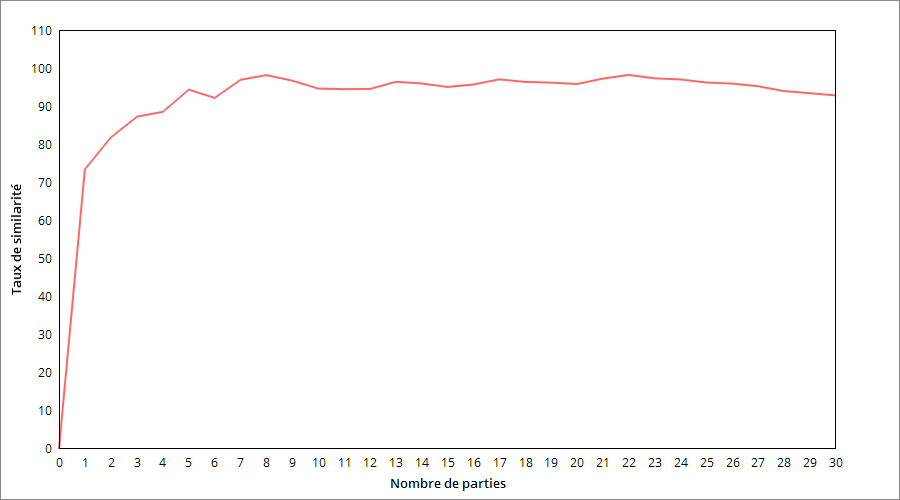
\includegraphics[scale=0.5]{./imagesRapport/profilageScenariosTestsAnalyseResultats.png}
	\caption{Taux de similarité du profilage en fonction du nombre de partie}
\end{figure}


Afin de pouvoir obtenir des résultats facilement observables et pouvoir les étudier, nous avons également produit des graphes comparant le profilage établi et le calibrage à déterminer du joueur en fonction du nombre de parties. La figure suivante correspond à un exemple de graphe dans lequel un adversaire agressif à 52\% et rationnel à 64\% est profilé. Comme nous pouvons le voir, les courbes d'agressivité et de rationalité correspondant au profil global établi au fur et à mesure des parties ont tendance à converger vers le profil réel. \\


\begin{figure}[H]
\begin{center}
	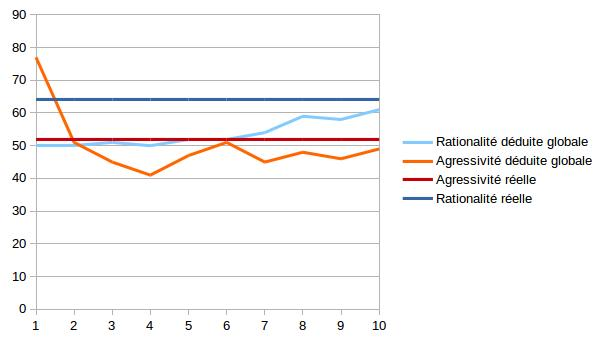
\includegraphics[scale=0.5]{./imagesRapport/profilEtabliEnFonctionPartiesEtReel.jpg}
	\caption{Profil établi en fonction du nombre de parties}
\end{center}
\end{figure}



Finalement, après avoir lancé un nombre important de parties, nous avons conçu le tableau suivant représentant le taux de similarité moyen obtenu pour chaque palier.

\begin{figure}[H]
\begin{center}
\begin{tabular}{|l|l|l|l|}
	\hline
	Palier d'agressivité & Palier de rationalité &	Taux de similarité moyen\\
\hline
0-40	 			    & 0-40 				 & 	69\%\\
\hline
0-40					&	40-60			 &	85\%\\
\hline
0-40					& 60-100				 &	82\%\\
\hline
40-60				&	0-40				 &	76\%\\
\hline
40-60				&	40-60			&	89\%\\
\hline
40-60				&	60-100			&	87\%\\
\hline
60-100				&	0-40				&	70\%\\
\hline
60-100				&	40-60			&	85\%\\
\hline
60-100				&	60-100			&	78\%\\

   \hline
\end{tabular}	
\end{center}
\caption{Taux de similarité des profils établis en fonction des paliers}
\end{figure}

Comme on peut le constater, on profile assez bien tous les types de joueurs. Les joueurs que nous arrivons le moins à profiler sont ceux ayant un taux de rationalité et un taux d'agressivité compris entre 0\% et 40\%. En effet, il est difficile de profiler un joueur qui aura tendance à jouer de manière irrationnelle, donc de manière très imprévisible. Ce type de joueur pourra alors miser fortement lorsqu'il n'a pas un bon jeu et miser peu lorsqu'il a un bon jeu. De plus, ce joueur étant à la fois irrationnel et peu agressif, nous obtenons des résultats pas forcément en accord avec les deux paramètres. Si le joueur a un mauvais jeu et qu'il joue de manière irrationnelle, il va miser fortement cependant, il n'est pas censé être agressif donc son taux d'agressivité s'en trouvera augmenté.\par


\section{Établissement des profils attendus}

\hspace{0.5cm}Pour calculer une action attendue, c'est à dire un taux d'agressivité et de rationalité attendu pour le joueur, l'intelligence artificielle utilise lors des premières parties les scénarios de tests établis.\par
Une fois le profilage lancé, et les premiers résultats obtenus, la méthode de profilage peut alors commencer à se servir des situations précédentes pour calculer l'action attendue d'un joueur de façon plus précise. En effet, selon la situation, il est possible de déterminer quelle va être l'action du joueur en se référant aux scénarios de tests conçus, qui sont communs à tous les joueurs, mais également en se référant aux parties précédentes, si l'on a déjà testé sa réaction précédemment dans une situation équivalente. Les scénarios de tests sont alors mis à jour de façon dynamique.\\

Pour reconnaître une situation équivalente, nous considérons le taux d'agressivité du joueur adverse, donc l'intelligence artificielle qui profile, et des chances de gain du joueur. A partir de cette méthode, la valeur d'une action réelle dans une situation va permettre de donner la valeur d'une action attendue dans une prochaine partie. Cette méthode va ici nous permettre de profiler le joueur plus rapidement, en réutilisant les résultats précédents.\\

Pour effectuer cette réutilisation, plusieurs méthodes ont été considérées. Tout d'abord, celle qui cherche la situation la plus proche, selon l'agressivité du profileur et les chances de gain, sans considérer le taux de similarité entre les deux situations. C'est à dire que dans cette version, les valeurs de l'action attendue correspondent aux valeurs des scénarios de tests uniquement pour la première partie. Par la suite, c'est la valeur précédente la plus proche qui est prise en compte, même si la situation n'est pas forcément similaire.\\

Par la suite, nous nous sommes rendus compte qu'il n'était pas optimal de reprendre une valeur précédente lorsque les paramètres de la partie étaient trop éloignés. Une seconde méthode a donc été de limiter la réutilisation des actions réelles comme actions attendues en considérant l'équivalence entre les parties. Toujours en prenant en compte les valeurs d'agressivité et des chances de gain, les pourcentages doivent alors ne varier que de 20\% maximum par exemple, pour que l'on puisse considérer la situation comme équivalente. Ici, on prend toujours la situation la plus proche, mais seulement parmi les parties dîtes équivalentes. Et donc dans le cas où les valeurs sont trop éloignées, on se réfère aux scénarios de tests de départ.\\

Nous avons également fait des tests en prenant en compte la situation dans laquelle la distance est la plus petite possible, c'est à dire prendre une situation dans laquelle l'intelligence artificielle a réussi à profiler correctement le joueur. Nous nous sommes rendus compte que la différence des résultats n'était pas significative, et qu'il valait mieux se baser sur les paramètres de la partie, à savoir le calibrage et les chances de gain de l'intelligence artificielle qui profile.\\

\section{Vérification du profil établi}

\hspace{0.5cm}Une fois le profil du joueur adverse établi, l'intelligence artificielle a pour but de jouer de façon à gagner le plus de jetons possible. Cependant, si le joueur adverse n'a pas été bien profilé, avec par exemple un profil à 40\% seulement, l'intelligence artificielle va jouer en imaginant jouer contre un type d'adversaire qui en fait n'est pas le bon. Par conséquent, nous avons choisi de mettre en place la possibilité de reprendre le profil afin de l’affiner si besoin. \\

Par conséquent si, lors de la phase de jeu et à partir de dix parties jouées, l'intelligence artificielle perd des jetons ou bien gagne moins de jetons que lors de la phase de scénarios de tests, l'intelligence artificielle reprend le profilage du joueur, en ne jouant donc plus pour gagner. Cette phase de reprise du profilage du joueur dure cinq parties. En effet, après avoir testé avec plusieurs nombres de parties différents, nous nous sommes rendus compte que cinq parties était largement suffisant. Par la suite, l'intelligence artificielle reprend sa phase de jeu pour gagner et, si au bout de dix parties, les gains ne sont toujours pas bons, l'intelligence artificielle recommence à profiler le joueur, et cætera.\\

\chapter{Analyse des gains de parties}

\hspace{0.5cm}Une fois un profil établi, nous pouvons alors faire jouer l'intelligence artificielle en fonction des résultats obtenus, dans le but de lui faire gagner le plus de jetons possibles. Lors de cette étape le profilage est interrompu, et on utilise le comportement déduit final pour calibrer l'intelligence artificielle de façon à ce qu'elle puisse gagner face à ce type de joueur.\par

\section{Un premier calibrage inefficace}

\subsection{Mise en place du calibrage}

\hspace{0.5cm}Pour une première version, nous avons choisi de seulement prendre en compte le profil final établi et d'attribuer un calibrage selon divers paliers. Ici on prend en compte trois paliers pour l'agressivité ainsi que pour la rationalité. De 0 à 40\% pour le premier palier, 40 à 60\% pour une valeur moyenne puis de 60 à 100\% pour la palier haut. Nous avons alors déduit les calibrages correspondants à chaque palier du joueur profilé, les résultats sont présentés dans le tableau suivant.\\
\begin{figure}[H]
\begin{center}
\begin{tabular}{|l|l|l|l|}
\hline
Agressivité déduite & Rationalité déduite &	Agressivité IA & 	Rationalité IA\\
\hline
0-40	 			    & 0-40 				 & 	70-100		   & 50\\
\hline
0-40					&	40-60			 &	50-70		   & 	50\\
\hline
0-40					& 60-100				 &	70-100		   &	30-50\\
\hline
40-60				&	0-40				 &	70-100		   &	50\\
\hline
40-60				&	40-60			&	70-100			&	30-50\\
\hline
40-60				&	60-100			&	50-70			&	70-90\\
\hline
60-100				&	0-40				&	50-70			&	70-90\\
\hline
60-100				&	40-60			&	70-100			&	50-70\\
\hline
60-100				&	60-100			&	50				&	90-100\\
\hline
\end{tabular}
\end{center}
\caption{Calibrage de l'intelligence artificielle en fonction du profil adverse}
\end{figure}


Le but de notre intelligence artificielle étant, une fois un profilage correctement établi, de pouvoir augmenter son gain de parties mais aussi son gain d'argent. Nous avons donc renseigné dans l'application le nombre de parties au bout desquelles l'intelligence artificielle va pouvoir arrêter le profilage, et donc adapter elle-même son calibrage pour pouvoir gagner un maximum de parties.\\

\subsection{Analyse des résultats}

\hspace{0.5cm}Afin de pouvoir étudier les gains de l'intelligence artificielle avant et après le profilage, nous avons alors ajouté dans les fichiers résultats le gain de parties et d'argent pour chacune des parties. Ceci nous a permis de pouvoir obtenir un ratio du nombre de parties gagnées sur le nombre de parties jouées pendant le profilage, puis pendant la phase de jeu. De même pour le nombre de jetons obtenus. Nous avons donc ajouté les lignes suivantes à la fin de chaque fichier contenant le profil établi.\\

\begin{figure}[H]
\begin{center}
\begin{tabular}{|l|l|l|l|}
\hline
Nombre de parties:&	30		\\
\hline
Nombre de parties gagnées par l'IA pendant profilage :& 6 sur 10\\
\hline
Nombre de parties gagnées par l'IA pendant jeu :& 15 sur 20\\
\hline
Gains de l'IA pendant profilage :& -924		\\
\hline
Gains de l'IA pendant jeu :&	3530		\\
\hline
\end{tabular}
\end{center}
\caption{Données situées à la fin d'un fichier contenant le profil établi d'un joueur}
\end{figure}

Ces données sont mises à jour à chaque nouvelle partie.\\


La figure suivante représente le nombre de parties gagnées pendant les scénarios de tests et le nombre de parties gagnées après, pour chaque type d'adversaire possible. Comme on peut le constater, le nombre de parties gagnées après le déroulement des scénarios de tests, donc lorsque l'intelligence artificielle qui profile joue en fonction des résultats obtenus, est meilleur. En effet, celle-ci gagne souvent plus de parties que lors de la période de scénarios de tests. \\


\begin{figure}[H]
	\begin{center}
		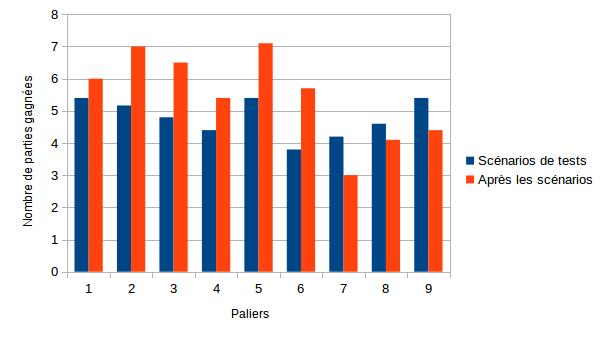
\includegraphics[scale=0.5]{./imagesRapport/PremierCalibrageComparaisonNombrePartiesGagnees.jpg}
		
		\hspace{-1.5cm}\begin{tabular}{|l|l|l|}
			\hline
			Palier & 	Agressivité &	Rationalité\\
			\hline
			 1 & 0-40 & 0-40\\
			\hline
			 2 & 	0-40 & 40-60\\
			\hline
			 3 & 0-40 & 60-100\\
			\hline
			 4 & 	40-60 & 0-40\\
			\hline
			 5 & 40-60 & 40-60\\
			\hline
			 6 & 40-60 & 60-100\\
			\hline
			 7 & 60-100 & 0-40\\
			\hline
			 8 & 60-100 & 40-60\\
			\hline
			 9 & 60-100 & 60-100\\
			\hline
		\end{tabular}
		
	\end{center}
	\caption{Nombre de parties gagnées pendant les scénarios de tests et après}
\end{figure}


Même si nous gagnons plus de parties que lors de la phase de scénarios de tests, nous avons remarqué que nous avons des gains nettement moins bons. En effet, comme on peut le voir dans la figure suivante représentant le nombre de jetons gagnés en moyenne pour chaque partie, les gains sont moins bons lors de la phase de jeu en fonction de profil. L'intelligence artificielle perd même des jetons dans la majorité des paliers. Ces mauvais résultats peuvent s'expliquer par le fait que nous avons mis en place des taux d'agressivité élevés en réponse aux différents profils établis. De ce fait, lorsque l'intelligence artificielle gagne des jetons, elle n'en gagne pas énormément car le joueur adverse va avoir tendance à se coucher rapidement étant donné qu'il sera effrayé par le fort taux d'agressivité. Cependant, lorsque l'intelligence artificielle perd des parties, étant agressive, elle aura auparavant mis en jeu beaucoup de jetons. Par conséquent, elle aura tendance à perdre plus de jetons qu'elle n'en gagne.\par


\begin{figure}[H]
	\begin{center}
		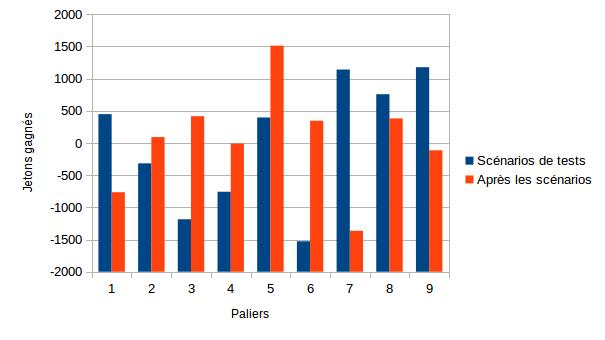
\includegraphics[scale=0.5]{./imagesRapport/PremierCalibrageComparaisonJetonsGagnees.jpg}
	\end{center}
	\caption{Nombre de jetons gagnés pendant les scénarios de tests et après}
\end{figure}


\section{Recherche du calibrage optimal}

\hspace{0.5cm}Puisque les premières réponses face à un profilage établi pour gagner le plus de parties et de jetons possibles n'étaient pas concluantes, nous avons établi des tests permettant de déterminer un calibrage optimal.\par
Pour cela, nous avons lancé une série de parties face à un profil donné en faisant varier le calibrage de l'intelligence artificielle qui profile. Nous avons fait varier chacun des paramètres, agressivité et rationalité, de 15 en 15 de la façon suivante.\\

\begin{center}
15 - 30 - 45 - 60 - 75 - 90 - 100
\end{center}


Nous avons ensuite effectué le produit cartésien entre les deux listes pour obtenir tous les calibrages possibles (par exemple 15-15, 15-30...). Puis pour chaque calibrage, nous avons lancé 100 parties.\par

Nous récupérions à la fin des 100 parties le taux de parties gagnées ainsi que le nombre de jetons gagnés ou perdus.\\

La figure suivante correspond au résultat de la recherche du calibrage optimal face à un joueur 80\% agressif et 80\% rationnel. Ainsi, la courbe bleue correspond au taux de parties gagnées alors que la seconde courbe correspond au nombre de jetons gagnés au total pendant les cent parties lancées par calibrage. L'abscisse correspond aux calibrages testés. Ainsi, le calibrage numéro un correspond au calibrage 15-15 alors que le dernier calibrage, à savoir le numéro 49, correspond au calibrage 100-100.   

Comme on peut le voir, la courbe du nombre de parties gagnées a tendance à croître de manière significative à partir du moment où on arrive aux calibrages ayant 75\% d'agressivité et plus. En effet, le joueur adverse étant calibré à 80\% d'agressivité et 80\% de rationalité, par conséquent, les joueurs étant moins agressifs gagnent moins souvent. Concernant les jetons gagnés, on constate que la courbe dans son ensemble ne semble pas avoir un comportement défini. 
On peut voir que les points les plus intéressant sont le point correspondant au calibrage numéro six, à savoir, un comportement 15\% agressif et 90\% rationnel, et le point correspondant au calibrage numéro 46, à savoir, un comportement 100\% agressif et 60\% rationnel. Le calibrage correspondant au point numéro six permet à l'intelligence artificielle de gagner environ 45\% des parties et 15 000 jetons. Cependant le point numéro 46 semble plus intéressant. En effet, avec ce calibrage, l'intelligence artificielle gagne, lors de sa phase de jeu, un nombre important de parties, à savoir, plus de 65\% de parties mais aussi un nombre important de jetons, à savoir, plus de 13 000 jetons. Finalement, nous avons choisi de calibrer notre intelligence artificielle à 100\% d'agressivité et 60\% de rationalité face à un joueur profilé avec un taux d'agressivité compris entre 60\% et 100\% et un taux de rationalité compris entre 60\% et 100\%. Ce calibrage correspond donc au calibrage numéro 46 décrit précédemment. \par


\begin{figure}[H]
	\begin{center}
		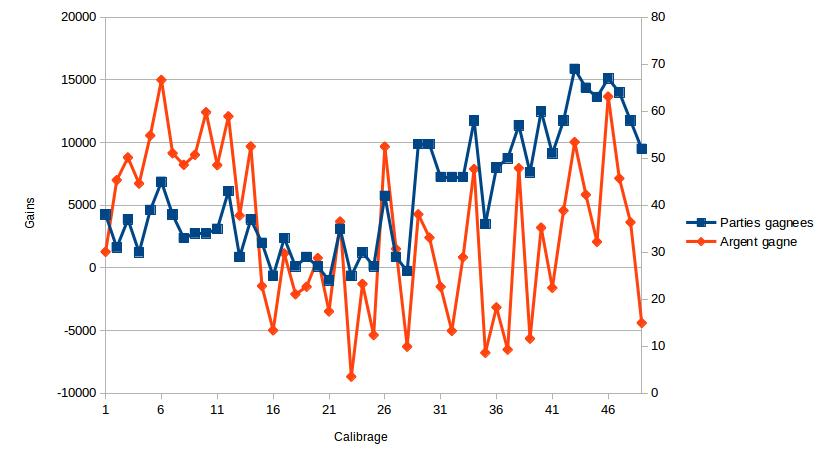
\includegraphics[scale=0.5]{./imagesRapport/rechercheCalibrageOptimal8080.jpg}
	\end{center}
	\caption{Gains en fonction du calibrage face à un joueur à 80\% agressif et 80\% rationnel}
\end{figure}


Après avoir effectué une première recherche du calibrage optimal pour un palier donné concluante, nous avons choisi de lancer cette recherche pour chacun des autres paliers, afin de permettre à notre intelligence artificielle d'avoir le meilleur jeu possible dans n'importe quelle situation.\par

Nous avons finalement choisi les calibrages suivants pour les différents paliers présentés ci-dessous.

\begin{figure}[H]
\begin{center}
\begin{tabular}{|l|l|l|l|}
\hline
Agressivité déduite &	Rationalité déduite &	Agressivité IA & 	Rationalité IA\\
\hline
0-40	 & 0-40 &	30 &	30\\
\hline
0-40 &	40-60 &	30 &	90-100\\
\hline
0-40	 & 60-100 &	15&	90-100\\
\hline
40-60 &	0-40 &	30 &	90\\
\hline
40-60 &	40-60 &	70-80 & 70-80\\
\hline
40-60 &	60-100 &	 90 &	30\\
\hline
60-100 &	 0-40 &	30 & 	90-100\\
\hline
60-100 & 	40-60 &	15 & 	75-100\\
\hline
60-100 &	 60-100 &	100 &	60\\
\hline
\end{tabular}
\end{center}
\caption{Calibrage final de l'intelligence artificielle en fonction du profil adverse}
\end{figure}


\begin{figure}[H]
	\begin{center}
		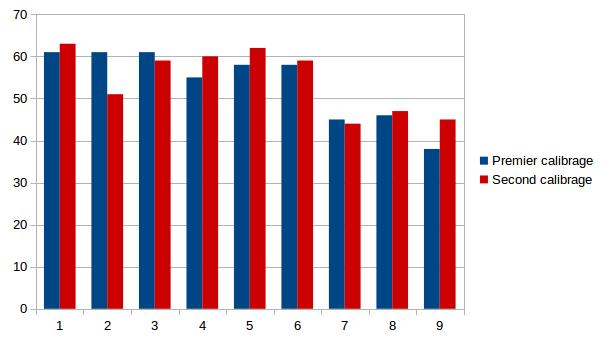
\includegraphics[scale=0.5]{./imagesRapport/NombrePartiesGagneesEnFonctionCalibrage.jpg}
	\end{center}
	\caption{Nombre de parties gagnées en fonction du premier calibrage établi et du second calibrage calculé}
\end{figure}

Comme on peut le voir dans la figure ci-dessus, le changement de gains de parties par rapport aux résultats précédents n'est pas énorme voire moins bon dans certains paliers. En effet, les données bleues et rouges, respectivement le premier calibrage établi inefficace et le second calibrage résultant de la recherche du calibrage optimal sont sensiblement égales. Nous avons choisi de nous concentrer davantage sur les gains de jetons. Ainsi, même si un l'intelligence artificielle qui profile ne gagne pas plus de parties, elle gagne plus de jetons qu’auparavant. Le diagramme suivant représente les jetons gagnés en fonction du premier calibrage établi, en bleu, et du second calibrage établi en fonction des données collectées pendant la recherche du calibrage optimal, en rouge. On constate rapidement que le nombre de jetons gagnés en moyenne sur une partie est nettement meilleur qu'auparavant. Notamment dans le premier palier, correspondant à un jeu face à une intelligence artificielle profilée avec une agressivité et une rationalité comprises entre 0\% et 40\%, où le nombre de jetons gagnés passe d'une perte de plus de 120 jetons en moyenne à un gain d'une trentaine de jetons en moyenne par partie. \\

\begin{figure}[H]
	\begin{center}
		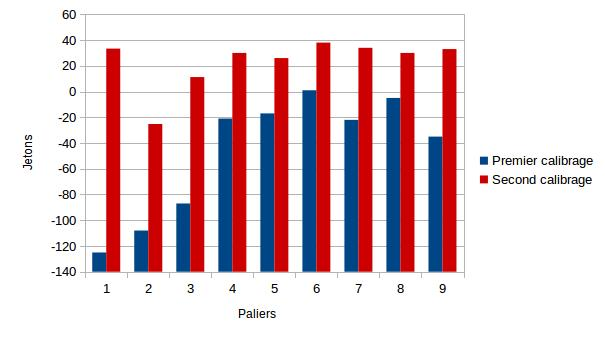
\includegraphics[scale=0.5]{./imagesRapport/JetonsGagnesEnFonctionCalibrage.jpg}
	\end{center}
	\caption{Nombre de parties gagnées en fonction des deux calibrages}
\end{figure}

La recherche de calibrages optimaux pour chacun des palier nous a donc permis d'améliorer de façon significative le nombre de jetons gagnés en moyenne par partie après établissement du profil de l'adversaire.

\section{Résultats}
\hspace{0.5cm}Suite à ces résultats, nous avons donc pu produire des courbes de gain en fonction du nombre de parties jouées, et aussi en fonction du mode de jeu de l'intelligence artificielle (profilage ou jeu pour gagner). Nous avons également pu afficher dans une même graphe entre les courbes de profilage et courbe de gain.\par
Dans le but de rendre plus significative la courbe de profilage, et donc de mieux voir la corrélation entre les deux courbes, nous avons modifié l'affichage de la courbe de profilage. En effet, selon le calibrage à déterminer, la variation de la courbe n'est pas la même. Nous avons donc fait en sorte que celle-ci corresponde à la différence entre le profilage établi et le calibrage réel. Ainsi, plus cette courbe diminue, plus le profilage établi est précis. Et donc plus cette courbe diminue, plus la courbe de gain est supposée augmenter.\\
 

\chapter{Perspectives et conclusion}
\section{Perspectives d'amélioration du profilage}
\subsection{Profilage dynamique}
\hspace{0.5cm}Même si nous n'avons pas eu le temps d'implémenter la méthode de profilage dynamique, nous avons pu réfléchir un peu à la façon de profiler dynamiquement un adversaire.\par
Premièrement, lors de la phase de scénarios de tests, nous n'établirions pas le profil uniquement à la fin de la partie mais plutôt au fur et à mesure de la partie, en se basant sur les actions qu'il a effectué en réponse à nos actions. De même, lors de la phase de scénarios de tests, plutôt que de définir au départ de la partie un calibrage fixe pour l'intelligence artificielle qui profile, nous pourrions choisir de modifier le calibrage en fonction des actions effectuées par le joueur pendant la partie. En effet, si l'on se rend vite compte que le joueur adverse a tendance à être agressif face à un joueur peu agressif, nous pourrions augmenter l'agressivité de l'intelligence artificielle qui profile afin de voir s'il répond toujours ou bien s'il a tendance à suivre. De ce fait, nous pourrions définir des paliers et rapidement savoir dans quel palier d'agressivité et de rationalité se trouve l'adversaire.\\

De plus, après les scénarios de tests, lors de la phase de gains, nous pourrions décider de faire en sorte que l'intelligence artificielle modifie son calibrage à chaque tour de jeu, en fonction de l'action jouée par le joueur adverse et de la situation du jeu, contrairement à la phase de gains actuelle, pour laquelle l'intelligence artificielle ne change pas de profil.\par

\subsection{Profilage avec plus de deux joueurs}
\hspace{0.5cm}Notre méthode de profilage étant actuellement basée sur un jeu à uniquement deux joueurs, on peut se poser la question d'un profilage sur un jeu à plus de deux joueurs. En effet, les paramètres à prendre en compte pour établir le profil d'un joueur adverse ne seraient pas les mêmes. Il faudrait par exemple ajouter dans ces paramètres le nombre de joueurs adverses, qui influence les comportements. Si un joueur a peu de chances de gain et un nombre important de joueurs adverses, il sera sûrement bien plus rationnel et aura sûrement plus tendance à se coucher que s'il avait été contre un seul adversaire. En effet, il y a plus de chances que ses joueurs adverses aient un meilleur jeu que lui. De même, un joueur ayant un jeu moyen et jouant de manière prudente n'aura sûrement pas le même comportement s'il est face à un ou plusieurs joueurs. De même, on peut penser que face à plusieurs adversaires, un joueur va prendre plus de risques pour rester dans le jeu et donc, être moins rationnel et plus agressif. De ce fait, dans un jeu à plusieurs joueurs, le nombre de joueurs serait un critère très important pour le calcul des taux d'agressivité, de rationalité, de bluff et de passivité d'un adversaire. \\
Dans le cas d'un profilage avec plusieurs adversaires, lors de la phase de scénarios de tests, l'intelligence artificielle n'aurait pas forcément besoin d'être agressive puisqu'il y aurait plus de joueurs donc possiblement des joueurs qui pourraient jouer de manière agressive pour elle. Par conséquent, l'intelligence artificielle pourrait faire en sorte de perdre moins de jetons pendant les parties de profilage tout en continuant à profiler les joueurs adverses.\par 


\section{Profilage obtenu}
\hspace{0.5cm}Au terme du projet, nous avons finalement obtenu un bon profilage statique. En effet, nous arrivons à profiler un joueur à 80\% près en moyenne au bout de quelques parties. Après avoir établi le profil, l'intelligence artificielle est capable de gagner plus de jetons que durant la phase de profilage. Cependant, on a pu constater que face à un joueur très irrationnel, il n'est pas facile pour nous de gagner beaucoup de jetons. En effet, il est très difficile de prédire les actions qui seront effectuées par un joueur irrationnel. Même si face à ce type de joueurs nous n'obtenons pas de résultats satisfaisants, nous obtenons dans l'ensemble des résultats très corrects pour la plupart des types de joueurs adverses.\par





%%bibliographie /sitographie

\bibliographystyle{plain}
\nocite{*}
\bibliography{biblio}

%%Annexes
\appendix
\chapter{Planification prévisionnelle}
		 \hspace{-4.2cm} 
			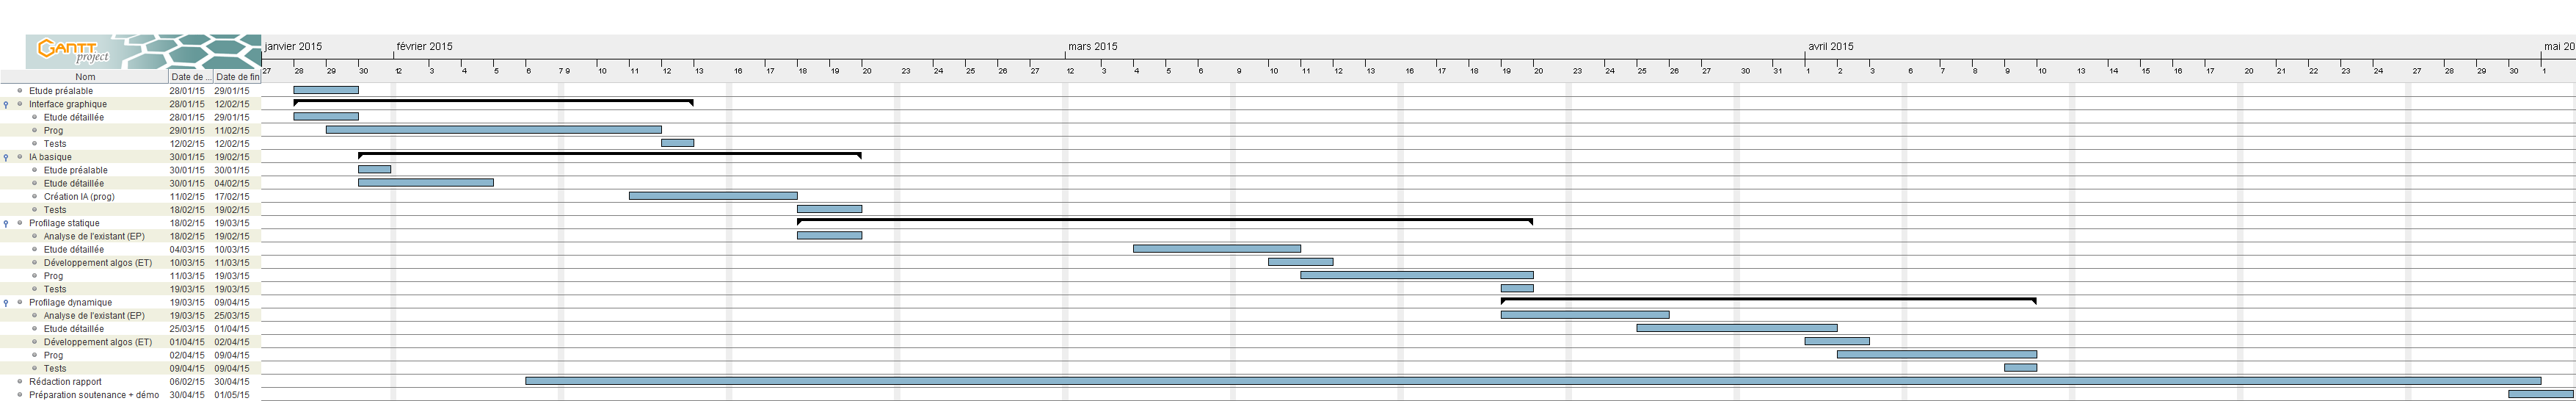
\includegraphics[scale=0.28]{../DiagrammePrevisionnel.png}
	\medskip
		
\chapter{Planification réelle}
		 \hspace{-4.5cm} 
			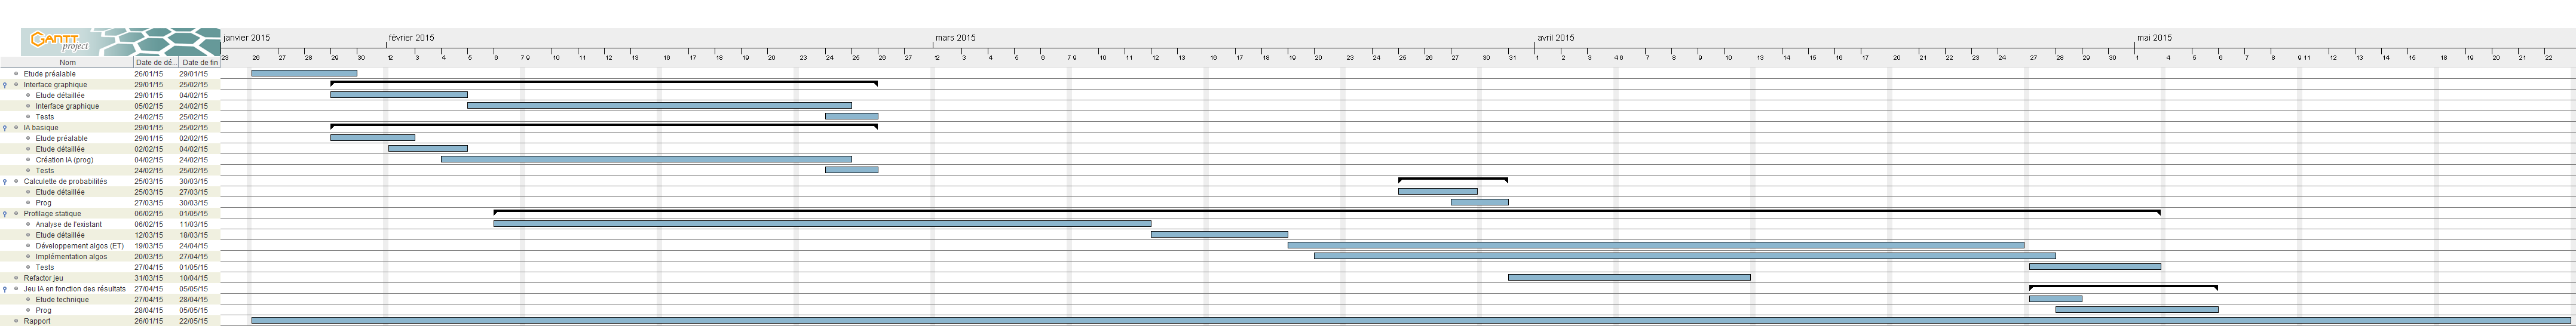
\includegraphics[scale=0.24]{../DiagrammeReel.png}

	\medskip
		
		
		
\end{document}
